% Options for packages loaded elsewhere
\PassOptionsToPackage{unicode}{hyperref}
\PassOptionsToPackage{hyphens}{url}
\PassOptionsToPackage{dvipsnames,svgnames,x11names}{xcolor}
%
\documentclass[
  letterpaper,
  DIV=11,
  numbers=noendperiod]{scrartcl}

\usepackage{amsmath,amssymb}
\usepackage{iftex}
\ifPDFTeX
  \usepackage[T1]{fontenc}
  \usepackage[utf8]{inputenc}
  \usepackage{textcomp} % provide euro and other symbols
\else % if luatex or xetex
  \usepackage{unicode-math}
  \defaultfontfeatures{Scale=MatchLowercase}
  \defaultfontfeatures[\rmfamily]{Ligatures=TeX,Scale=1}
\fi
\usepackage{lmodern}
\ifPDFTeX\else  
    % xetex/luatex font selection
\fi
% Use upquote if available, for straight quotes in verbatim environments
\IfFileExists{upquote.sty}{\usepackage{upquote}}{}
\IfFileExists{microtype.sty}{% use microtype if available
  \usepackage[]{microtype}
  \UseMicrotypeSet[protrusion]{basicmath} % disable protrusion for tt fonts
}{}
\makeatletter
\@ifundefined{KOMAClassName}{% if non-KOMA class
  \IfFileExists{parskip.sty}{%
    \usepackage{parskip}
  }{% else
    \setlength{\parindent}{0pt}
    \setlength{\parskip}{6pt plus 2pt minus 1pt}}
}{% if KOMA class
  \KOMAoptions{parskip=half}}
\makeatother
\usepackage{xcolor}
\setlength{\emergencystretch}{3em} % prevent overfull lines
\setcounter{secnumdepth}{-\maxdimen} % remove section numbering
% Make \paragraph and \subparagraph free-standing
\makeatletter
\ifx\paragraph\undefined\else
  \let\oldparagraph\paragraph
  \renewcommand{\paragraph}{
    \@ifstar
      \xxxParagraphStar
      \xxxParagraphNoStar
  }
  \newcommand{\xxxParagraphStar}[1]{\oldparagraph*{#1}\mbox{}}
  \newcommand{\xxxParagraphNoStar}[1]{\oldparagraph{#1}\mbox{}}
\fi
\ifx\subparagraph\undefined\else
  \let\oldsubparagraph\subparagraph
  \renewcommand{\subparagraph}{
    \@ifstar
      \xxxSubParagraphStar
      \xxxSubParagraphNoStar
  }
  \newcommand{\xxxSubParagraphStar}[1]{\oldsubparagraph*{#1}\mbox{}}
  \newcommand{\xxxSubParagraphNoStar}[1]{\oldsubparagraph{#1}\mbox{}}
\fi
\makeatother

\usepackage{color}
\usepackage{fancyvrb}
\newcommand{\VerbBar}{|}
\newcommand{\VERB}{\Verb[commandchars=\\\{\}]}
\DefineVerbatimEnvironment{Highlighting}{Verbatim}{commandchars=\\\{\}}
% Add ',fontsize=\small' for more characters per line
\usepackage{framed}
\definecolor{shadecolor}{RGB}{241,243,245}
\newenvironment{Shaded}{\begin{snugshade}}{\end{snugshade}}
\newcommand{\AlertTok}[1]{\textcolor[rgb]{0.68,0.00,0.00}{#1}}
\newcommand{\AnnotationTok}[1]{\textcolor[rgb]{0.37,0.37,0.37}{#1}}
\newcommand{\AttributeTok}[1]{\textcolor[rgb]{0.40,0.45,0.13}{#1}}
\newcommand{\BaseNTok}[1]{\textcolor[rgb]{0.68,0.00,0.00}{#1}}
\newcommand{\BuiltInTok}[1]{\textcolor[rgb]{0.00,0.23,0.31}{#1}}
\newcommand{\CharTok}[1]{\textcolor[rgb]{0.13,0.47,0.30}{#1}}
\newcommand{\CommentTok}[1]{\textcolor[rgb]{0.37,0.37,0.37}{#1}}
\newcommand{\CommentVarTok}[1]{\textcolor[rgb]{0.37,0.37,0.37}{\textit{#1}}}
\newcommand{\ConstantTok}[1]{\textcolor[rgb]{0.56,0.35,0.01}{#1}}
\newcommand{\ControlFlowTok}[1]{\textcolor[rgb]{0.00,0.23,0.31}{\textbf{#1}}}
\newcommand{\DataTypeTok}[1]{\textcolor[rgb]{0.68,0.00,0.00}{#1}}
\newcommand{\DecValTok}[1]{\textcolor[rgb]{0.68,0.00,0.00}{#1}}
\newcommand{\DocumentationTok}[1]{\textcolor[rgb]{0.37,0.37,0.37}{\textit{#1}}}
\newcommand{\ErrorTok}[1]{\textcolor[rgb]{0.68,0.00,0.00}{#1}}
\newcommand{\ExtensionTok}[1]{\textcolor[rgb]{0.00,0.23,0.31}{#1}}
\newcommand{\FloatTok}[1]{\textcolor[rgb]{0.68,0.00,0.00}{#1}}
\newcommand{\FunctionTok}[1]{\textcolor[rgb]{0.28,0.35,0.67}{#1}}
\newcommand{\ImportTok}[1]{\textcolor[rgb]{0.00,0.46,0.62}{#1}}
\newcommand{\InformationTok}[1]{\textcolor[rgb]{0.37,0.37,0.37}{#1}}
\newcommand{\KeywordTok}[1]{\textcolor[rgb]{0.00,0.23,0.31}{\textbf{#1}}}
\newcommand{\NormalTok}[1]{\textcolor[rgb]{0.00,0.23,0.31}{#1}}
\newcommand{\OperatorTok}[1]{\textcolor[rgb]{0.37,0.37,0.37}{#1}}
\newcommand{\OtherTok}[1]{\textcolor[rgb]{0.00,0.23,0.31}{#1}}
\newcommand{\PreprocessorTok}[1]{\textcolor[rgb]{0.68,0.00,0.00}{#1}}
\newcommand{\RegionMarkerTok}[1]{\textcolor[rgb]{0.00,0.23,0.31}{#1}}
\newcommand{\SpecialCharTok}[1]{\textcolor[rgb]{0.37,0.37,0.37}{#1}}
\newcommand{\SpecialStringTok}[1]{\textcolor[rgb]{0.13,0.47,0.30}{#1}}
\newcommand{\StringTok}[1]{\textcolor[rgb]{0.13,0.47,0.30}{#1}}
\newcommand{\VariableTok}[1]{\textcolor[rgb]{0.07,0.07,0.07}{#1}}
\newcommand{\VerbatimStringTok}[1]{\textcolor[rgb]{0.13,0.47,0.30}{#1}}
\newcommand{\WarningTok}[1]{\textcolor[rgb]{0.37,0.37,0.37}{\textit{#1}}}

\providecommand{\tightlist}{%
  \setlength{\itemsep}{0pt}\setlength{\parskip}{0pt}}\usepackage{longtable,booktabs,array}
\usepackage{calc} % for calculating minipage widths
% Correct order of tables after \paragraph or \subparagraph
\usepackage{etoolbox}
\makeatletter
\patchcmd\longtable{\par}{\if@noskipsec\mbox{}\fi\par}{}{}
\makeatother
% Allow footnotes in longtable head/foot
\IfFileExists{footnotehyper.sty}{\usepackage{footnotehyper}}{\usepackage{footnote}}
\makesavenoteenv{longtable}
\usepackage{graphicx}
\makeatletter
\def\maxwidth{\ifdim\Gin@nat@width>\linewidth\linewidth\else\Gin@nat@width\fi}
\def\maxheight{\ifdim\Gin@nat@height>\textheight\textheight\else\Gin@nat@height\fi}
\makeatother
% Scale images if necessary, so that they will not overflow the page
% margins by default, and it is still possible to overwrite the defaults
% using explicit options in \includegraphics[width, height, ...]{}
\setkeys{Gin}{width=\maxwidth,height=\maxheight,keepaspectratio}
% Set default figure placement to htbp
\makeatletter
\def\fps@figure{htbp}
\makeatother

\KOMAoption{captions}{tableheading}
\makeatletter
\@ifpackageloaded{caption}{}{\usepackage{caption}}
\AtBeginDocument{%
\ifdefined\contentsname
  \renewcommand*\contentsname{Table of contents}
\else
  \newcommand\contentsname{Table of contents}
\fi
\ifdefined\listfigurename
  \renewcommand*\listfigurename{List of Figures}
\else
  \newcommand\listfigurename{List of Figures}
\fi
\ifdefined\listtablename
  \renewcommand*\listtablename{List of Tables}
\else
  \newcommand\listtablename{List of Tables}
\fi
\ifdefined\figurename
  \renewcommand*\figurename{Figure}
\else
  \newcommand\figurename{Figure}
\fi
\ifdefined\tablename
  \renewcommand*\tablename{Table}
\else
  \newcommand\tablename{Table}
\fi
}
\@ifpackageloaded{float}{}{\usepackage{float}}
\floatstyle{ruled}
\@ifundefined{c@chapter}{\newfloat{codelisting}{h}{lop}}{\newfloat{codelisting}{h}{lop}[chapter]}
\floatname{codelisting}{Listing}
\newcommand*\listoflistings{\listof{codelisting}{List of Listings}}
\makeatother
\makeatletter
\makeatother
\makeatletter
\@ifpackageloaded{caption}{}{\usepackage{caption}}
\@ifpackageloaded{subcaption}{}{\usepackage{subcaption}}
\makeatother

\ifLuaTeX
  \usepackage{selnolig}  % disable illegal ligatures
\fi
\usepackage{bookmark}

\IfFileExists{xurl.sty}{\usepackage{xurl}}{} % add URL line breaks if available
\urlstyle{same} % disable monospaced font for URLs
\hypersetup{
  pdftitle={DH 302 Spring 2025 Assignment 02},
  pdfauthor={Mradul Sonkar (23B0980)},
  colorlinks=true,
  linkcolor={blue},
  filecolor={Maroon},
  citecolor={Blue},
  urlcolor={Blue},
  pdfcreator={LaTeX via pandoc}}


\title{DH 302 Spring 2025 Assignment 02}
\usepackage{etoolbox}
\makeatletter
\providecommand{\subtitle}[1]{% add subtitle to \maketitle
  \apptocmd{\@title}{\par {\large #1 \par}}{}{}
}
\makeatother
\subtitle{The assignment is based on
\href{https://docs.google.com/presentation/d/15kxh03hVBR1ybnuBBvbT5pfInju1IVkmVH1trWbKJn4/edit?usp=sharing}{Lecture
7},
\href{https://docs.google.com/presentation/d/1ilRr6T5N26kLWjIoP-ttUbXLsKxCW8SFx92DAf-R8zA/edit?usp=sharing}{Lecture
8},
\href{https://docs.google.com/presentation/d/1vc9WxkdTmCMudnAxxe6cFRUyRALaN0CQ8ixm3Np4IXU/edit?usp=sharing}{Lecture
9}, and
\href{https://docs.google.com/presentation/d/1VT9ynRKMkdEBG9ysfBDhZR1c0DZ_UZ9Vvvzci22lbuw/edit?usp=sharing}{Lecture
10}. Due at 11:59PM (IST), Tuesday \(18^{th}\) February, 2025 via
Gradescope. Raw template is available
\href{https://drive.google.com/file/d/1RvXnFnPkDVPGGwllD187HW0MkutruZJv/view?usp=sharing}{here}
and an upto date version of this pdf is available
\href{https://drive.google.com/file/d/1RvXnFnPkDVPGGwllD187HW0MkutruZJv/view?usp=sharing}{here}.
Total points = 150}
\author{Mradul Sonkar (23B0980)}
\date{}

\begin{document}
\maketitle


\section{Instructions}\label{instructions}

Submit your solutions via
\href{https://www.gradescope.com/courses/946202}{gradescope} by 11:59 PM
(IST) Tuesday, \(18^{th}\) February 2025. In-person submissions will not
be entertained. Please upload a single PDF file. Late submissions are
allowed with a 10\% per day penalty (only upto 22nd February). You can
raise your questions related to the assignment on
\href{https://piazza.com/class/m5k3nf7l4e91cg/post/m6alu8nsltc1pq}{Piazza}
- please tag these as \texttt{assignment\_02}.

\begin{itemize}
\tightlist
\item
  For theory questions, you can either write your response for in latex
  or put a screenshot/picture of your handwritten response in the
  appropriate section. To embed scanned images, use this format:
  \texttt{!{[}question1{]}(/path/to/question1.png)} where
  \texttt{/path/to/question1.png} is the local path (on your laptop) to
  your scanned (handwritten) response to question1.
\item
  If you are writing the solutions for theory questions by hand please
  use a pen. Pencil submissions are difficult to read when scanned. You
  will have to take a scan for each such answer and embed it in this
  document.
\item
  Your final submission has to be the PDF that comes from this template
  - one single pdf. No Exceptions.
\item
  Please mention the name(s) of people you collaborated with and what
  exactly you discussed.
\end{itemize}

\textbf{Making your submission:} Raw template is available
\href{https://drive.google.com/file/d/1RvXnFnPkDVPGGwllD187HW0MkutruZJv/view?usp=sharing}{here}
and an upto date version of this pdf is available
\href{https://drive.google.com/file/d/1RvXnFnPkDVPGGwllD187HW0MkutruZJv/view?usp=sharing}{here}.
Open the template in Rstudio (you will need to ensure Quarto is
installed). Once you are done with your answers, use the ``render''
(arrow like) button on the toolbar to create a pdf. Only pdf submissions
are allowed.

\begin{Shaded}
\begin{Highlighting}[]
\CommentTok{\# theme for plots}
\NormalTok{theme }\OtherTok{\textless{}{-}} \FunctionTok{theme}\NormalTok{(}
    \AttributeTok{axis.line =} \FunctionTok{element\_line}\NormalTok{(}\AttributeTok{color =}\NormalTok{ scales}\SpecialCharTok{::}\FunctionTok{alpha}\NormalTok{(}\StringTok{"black"}\NormalTok{, }\FloatTok{0.5}\NormalTok{)),}
    \AttributeTok{axis.ticks =} \FunctionTok{element\_line}\NormalTok{(}\AttributeTok{color =}\NormalTok{ scales}\SpecialCharTok{::}\FunctionTok{alpha}\NormalTok{(}\StringTok{"black"}\NormalTok{, }\FloatTok{0.5}\NormalTok{)),}
    \AttributeTok{axis.title.x =} \FunctionTok{element\_text}\NormalTok{(}\AttributeTok{size =} \DecValTok{14}\NormalTok{, }
                                \AttributeTok{color =}\NormalTok{ scales}\SpecialCharTok{::}\FunctionTok{alpha}\NormalTok{(}\StringTok{"black"}\NormalTok{, }\FloatTok{0.5}\NormalTok{),}
                                \AttributeTok{margin =} \FunctionTok{margin}\NormalTok{(}\AttributeTok{t =} \DecValTok{10}\NormalTok{)),}
    \AttributeTok{axis.title.y =} \FunctionTok{element\_text}\NormalTok{(}\AttributeTok{size =} \DecValTok{14}\NormalTok{, }
                                \AttributeTok{color =}\NormalTok{ scales}\SpecialCharTok{::}\FunctionTok{alpha}\NormalTok{(}\StringTok{"black"}\NormalTok{, }\FloatTok{0.5}\NormalTok{),}
                                \AttributeTok{margin =} \FunctionTok{margin}\NormalTok{(}\AttributeTok{r =} \DecValTok{15}\NormalTok{)),}
    \AttributeTok{axis.text =} \FunctionTok{element\_text}\NormalTok{(}\AttributeTok{size =} \DecValTok{10}\NormalTok{, }\AttributeTok{color =} \StringTok{"black"}\NormalTok{) }
\NormalTok{  )}
\end{Highlighting}
\end{Shaded}

\section{Problem 01 {[}25 points{]}}\label{problem-01-25-points}

\textbf{Quality of life:} Improvement in quality of life was measured
for a group of heart disease patients after 8 weeks in an exercise
program. This experimental group was compared to a control group who
were not in the exercise program. Quality of life was measured using a
21-item questionnaire, with scores of 1--5 on each item. The improvement
data are as follows and are plotted below.

\begin{figure}[H]

{\centering \includegraphics{Assignment02_P1.png}

}

\caption{Problem 1 image is available
\href{https://drive.google.com/file/d/1ymDEesi6CjrMZvxZDIEDGxEwxbVw17Lo/view?usp=sharing}{here}}

\end{figure}%

\paragraph{1a. What is the null hypothesis? {[}2.5
points{]}}\label{a.-what-is-the-null-hypothesis-2.5-points}

\textbf{Answer:}

\(H_0\) : The mean improvement score for the people who joined the
exercise program and people who didn't is the same.

\[
H_{experimental} = H_{control}
\]

\paragraph{1b. What conclusion could you draw from the dotplot? {[}2.5
points{]}}\label{b.-what-conclusion-could-you-draw-from-the-dotplot-2.5-points}

\textbf{Answer:}

From the plot, it appears that the mean and the variance of data in both
the clusters is almost the same. Although, to draw any conclusion, we
need to perform some statistical tests.

\paragraph{1c. Here is computer output for a t test. Explain what the
P-value means in the context of this study. {[}5
points{]}}\label{c.-here-is-computer-output-for-a-t-test.-explain-what-the-p-value-means-in-the-context-of-this-study.-5-points}

\emph{t = 2.505, df = 33.23, p-value = 0.00866 alternative hypothesis:
true difference in means is greater than 0}

\textbf{Answer:}

Since the \(p-value\) is \(0.00866\), which is less than our
significance level (say \(0.05\)), we can \textbf{reject} the null
hypothesis. We accept that exercise program has a positive impact on the
improvement score.

\paragraph{\texorpdfstring{1d. If type-1 error \(\alpha = 0.01\), what
is your conclusion regarding \(H_0\)? State your conclusion in the
specific context of this problem. {[}5
points{]}}{1d. If type-1 error \textbackslash alpha = 0.01, what is your conclusion regarding H\_0? State your conclusion in the specific context of this problem. {[}5 points{]}}}\label{d.-if-type-1-error-alpha-0.01-what-is-your-conclusion-regarding-h_0-state-your-conclusion-in-the-specific-context-of-this-problem.-5-points}

\textbf{Answer:}

The probability of rejecting the null hypothesis when it's actually true
is very less, \(\alpha = 0.01\). So it is very unlikely that we
incorrectly rejected the null hypothesis and exercise program indeed
makes a positive impact on recovery.

\paragraph{1e. The computer output in part (c) is for the directional
test. What is the P-value for the nondirectional test? {[}5
points{]}}\label{e.-the-computer-output-in-part-c-is-for-the-directional-test.-what-is-the-p-value-for-the-nondirectional-test-5-points}

\textbf{Answer:}

The \(p-value\) for non-directional test is just going to be double of
the \(p-value\) of directional test. So,

\[
p' = 2 \times p = 2 \times 0.00866 = 0.01732
\]

\paragraph{\texorpdfstring{1f. If the test were nondirectional, and
\(\alpha\)= 0.01, what conclusions would we make? {[}5
points{]}}{1f. If the test were nondirectional, and \textbackslash alpha= 0.01, what conclusions would we make? {[}5 points{]}}}\label{f.-if-the-test-were-nondirectional-and-alpha-0.01-what-conclusions-would-we-make-5-points}

\textbf{Answer:}

In the above setting, \(p-value\) turns out to be greater than the
significant level, hence we fail to reject the null hypothesis. We don't
have enough evidence to say that exercising makes any difference in
improvement score of the patients.

\section{Problem 02 {[}10 points{]}}\label{problem-02-10-points}

\textbf{Normality goes for a toss:} Researchers took skin samples from
10 patients who had breast implants and from a control group of 6
patients. They recorded the level of interleukin-6 or IL6 in
picogram/ml/10 g of tissue, a measure of tissue inflammation, after each
tissue sample was cultured for 24 hours. The dataset is available below
(in R)

\begin{Shaded}
\begin{Highlighting}[]
\NormalTok{il6.breast.implant.patients }\OtherTok{\textless{}{-}} \FunctionTok{c}\NormalTok{(}\DecValTok{231}\NormalTok{, }\DecValTok{308287}\NormalTok{, }\DecValTok{33291}\NormalTok{, }\DecValTok{124550}\NormalTok{, }\DecValTok{17075}\NormalTok{,}
                                 \DecValTok{22955}\NormalTok{, }\DecValTok{95102}\NormalTok{, }\DecValTok{5649}\NormalTok{, }\DecValTok{840585}\NormalTok{, }\DecValTok{58924}\NormalTok{)}
\NormalTok{il6.control.patients }\OtherTok{\textless{}{-}} \FunctionTok{c}\NormalTok{(}\DecValTok{35324}\NormalTok{, }\DecValTok{12457}\NormalTok{, }\DecValTok{8276}\NormalTok{, }\DecValTok{44}\NormalTok{, }\DecValTok{278}\NormalTok{, }\DecValTok{840}\NormalTok{)}
\NormalTok{df.breast }\OtherTok{\textless{}{-}} \FunctionTok{data.frame}\NormalTok{(}\AttributeTok{value =}\NormalTok{ il6.breast.implant.patients)}
\NormalTok{df.control }\OtherTok{\textless{}{-}} \FunctionTok{data.frame}\NormalTok{(}\AttributeTok{value =}\NormalTok{ il6.control.patients)}
\end{Highlighting}
\end{Shaded}

\paragraph{2a. Draw a boxplot, violin and ridgeline plot {[}5
points{]}}\label{a.-draw-a-boxplot-violin-and-ridgeline-plot-5-points}

\begin{Shaded}
\begin{Highlighting}[]
\CommentTok{\# YOUR RESPONSE HERE}
\CommentTok{\# OUTPUT should be 3 plots}
\CommentTok{\# While making it with the defaults but correctly which fetch you full points}
\CommentTok{\# you can go the extra mile and show someone the creativ side of you}
\CommentTok{\# good colors, good scaling, good lines, showing all data points, adding a legend}
\FunctionTok{library}\NormalTok{(ggplot2)}
\FunctionTok{library}\NormalTok{(ggridges)}

\CommentTok{\# YOUR CODE HERE}

\NormalTok{df.breast}\SpecialCharTok{$}\NormalTok{group }\OtherTok{\textless{}{-}} \StringTok{"Breast"}
\NormalTok{df.control}\SpecialCharTok{$}\NormalTok{group }\OtherTok{\textless{}{-}} \StringTok{"Control"}

\NormalTok{df }\OtherTok{\textless{}{-}} \FunctionTok{rbind}\NormalTok{(df.breast, df.control) }\CommentTok{\# combining the dataframes for plotting}
\end{Highlighting}
\end{Shaded}

\begin{Shaded}
\begin{Highlighting}[]
\CommentTok{\# box plot}
\FunctionTok{ggplot}\NormalTok{(df, }\FunctionTok{aes}\NormalTok{(}\AttributeTok{x =}\NormalTok{ group, }\AttributeTok{y =}\NormalTok{ value, }\AttributeTok{fill =}\NormalTok{ group)) }\SpecialCharTok{+}
  \FunctionTok{scale\_fill\_manual}\NormalTok{(}\AttributeTok{values =} \FunctionTok{c}\NormalTok{(}\StringTok{"Breast"} \OtherTok{=} \StringTok{"lightblue"}\NormalTok{, }\StringTok{"Control"} \OtherTok{=} \StringTok{"pink"}\NormalTok{)) }\SpecialCharTok{+} 
  \FunctionTok{scale\_y\_log10}\NormalTok{() }\SpecialCharTok{+} \CommentTok{\# i am using log10 scaled y{-}axis}
  \FunctionTok{geom\_boxplot}\NormalTok{(}\AttributeTok{color =}\NormalTok{ scales}\SpecialCharTok{::}\FunctionTok{alpha}\NormalTok{(}\StringTok{"black"}\NormalTok{, }\FloatTok{0.5}\NormalTok{)) }\SpecialCharTok{+}
  \FunctionTok{theme\_minimal}\NormalTok{() }\SpecialCharTok{+}
  \FunctionTok{labs}\NormalTok{(}\AttributeTok{title =} \StringTok{"IL{-}6 Levels in Breast Implant vs Control Patients"}\NormalTok{,}
       \AttributeTok{x =} \StringTok{"Patient Group"}\NormalTok{,}
       \AttributeTok{y =} \StringTok{"IL{-}6 Level (log10 scaled)"}\NormalTok{,}
       \AttributeTok{fill =} \StringTok{"Group"}\NormalTok{) }\SpecialCharTok{+}
\NormalTok{  theme}
\end{Highlighting}
\end{Shaded}

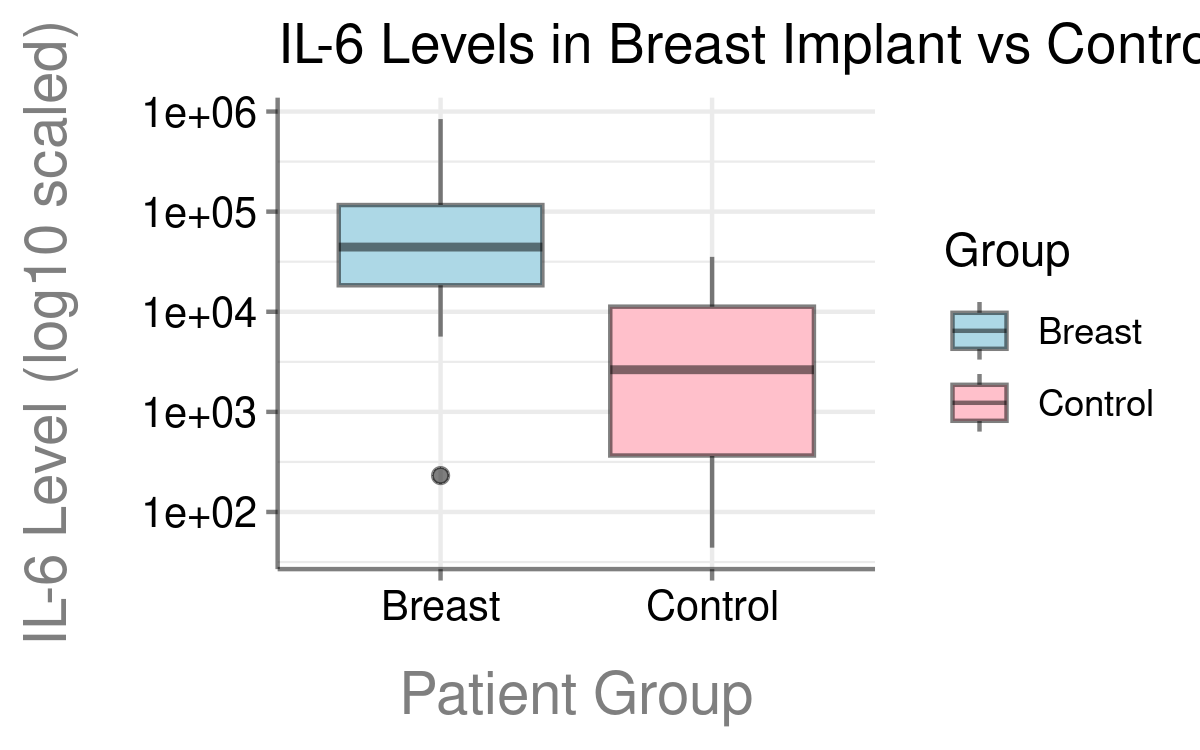
\includegraphics{DH302_Spring2025_Assignment02_files/figure-pdf/unnamed-chunk-5-1.png}

\begin{Shaded}
\begin{Highlighting}[]
\CommentTok{\# violin plot}
\FunctionTok{ggplot}\NormalTok{(df, }\FunctionTok{aes}\NormalTok{(}\AttributeTok{x =}\NormalTok{ group, }\AttributeTok{y =}\NormalTok{ value, }\AttributeTok{fill =}\NormalTok{ group)) }\SpecialCharTok{+}
  \FunctionTok{geom\_violin}\NormalTok{(}\AttributeTok{trim =} \ConstantTok{FALSE}\NormalTok{, }\AttributeTok{alpha=}\FloatTok{0.8}\NormalTok{, }\AttributeTok{color =}\NormalTok{ scales}\SpecialCharTok{::}\FunctionTok{alpha}\NormalTok{(}\StringTok{"black"}\NormalTok{, }\FloatTok{0.3}\NormalTok{)) }\SpecialCharTok{+}
  \FunctionTok{scale\_y\_log10}\NormalTok{() }\SpecialCharTok{+} \CommentTok{\# again i am using log10 scaled y{-}axis}
  \FunctionTok{theme\_minimal}\NormalTok{() }\SpecialCharTok{+}
  \FunctionTok{scale\_fill\_manual}\NormalTok{(}\AttributeTok{values =} \FunctionTok{c}\NormalTok{(}\StringTok{"Breast"} \OtherTok{=} \StringTok{"lightblue"}\NormalTok{, }\StringTok{"Control"} \OtherTok{=} \StringTok{"pink"}\NormalTok{)) }\SpecialCharTok{+} 
  \FunctionTok{labs}\NormalTok{(}\AttributeTok{title =} \StringTok{"IL{-}6 Levels in Breast Implant vs Control Patients"}\NormalTok{,}
       \AttributeTok{x =} \StringTok{"Patient Group"}\NormalTok{,}
       \AttributeTok{y =} \StringTok{"IL{-}6 Level (log10 scaled)"}\NormalTok{,}
       \AttributeTok{fill =} \StringTok{"Group"}\NormalTok{) }\SpecialCharTok{+}
\NormalTok{  theme}
\end{Highlighting}
\end{Shaded}

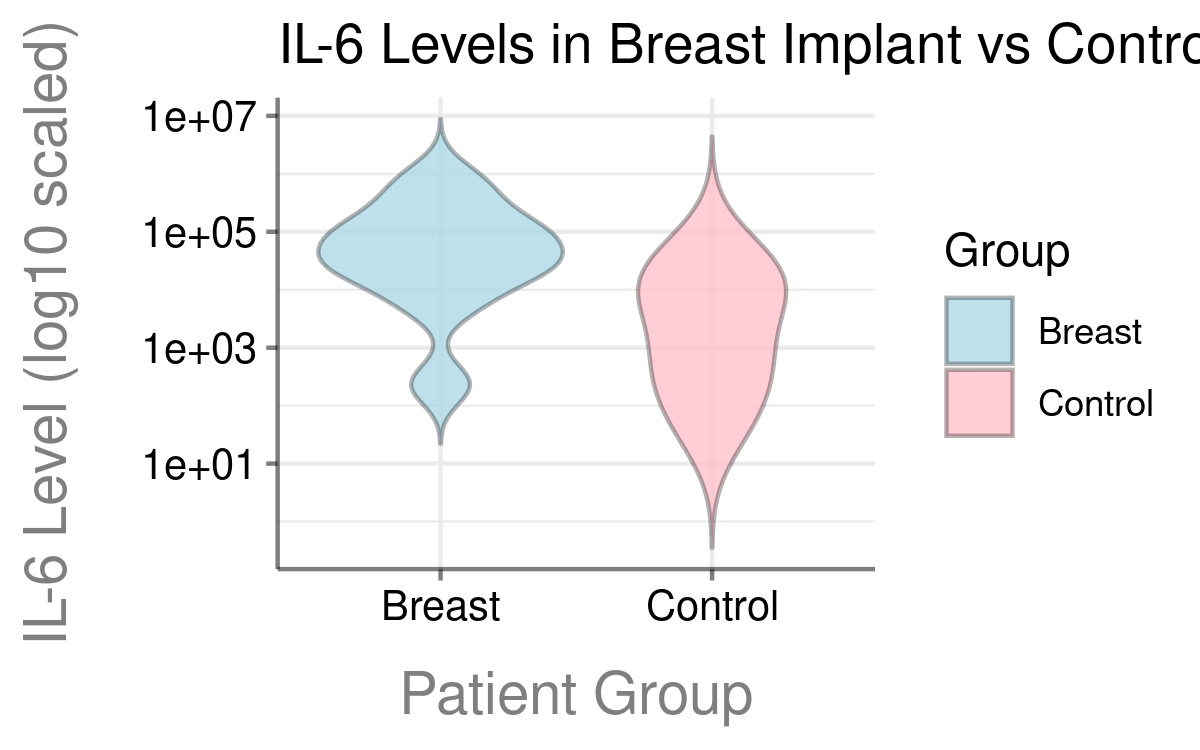
\includegraphics{DH302_Spring2025_Assignment02_files/figure-pdf/unnamed-chunk-6-1.png}

\begin{Shaded}
\begin{Highlighting}[]
\CommentTok{\# ridgeline plot}
\FunctionTok{ggplot}\NormalTok{(df, }\FunctionTok{aes}\NormalTok{(}\AttributeTok{x =}\NormalTok{ value, }\AttributeTok{y =}\NormalTok{ group, }\AttributeTok{fill =}\NormalTok{ group)) }\SpecialCharTok{+}
  \FunctionTok{geom\_density\_ridges}\NormalTok{(}\AttributeTok{alpha =} \FloatTok{0.7}\NormalTok{, }\AttributeTok{color =}\NormalTok{ scales}\SpecialCharTok{::}\FunctionTok{alpha}\NormalTok{(}\StringTok{"black"}\NormalTok{, }\FloatTok{0.3}\NormalTok{)) }\SpecialCharTok{+}
  \FunctionTok{theme\_minimal}\NormalTok{() }\SpecialCharTok{+}
  \FunctionTok{scale\_fill\_manual}\NormalTok{(}\AttributeTok{values =} \FunctionTok{c}\NormalTok{(}\StringTok{"Breast"} \OtherTok{=} \StringTok{"lightblue"}\NormalTok{, }\StringTok{"Control"} \OtherTok{=} \StringTok{"pink"}\NormalTok{)) }\SpecialCharTok{+} 
  \FunctionTok{labs}\NormalTok{(}\AttributeTok{title =} \StringTok{"IL{-}6 Levels in Breast Implant vs Control Patients"}\NormalTok{,}
        \AttributeTok{x =} \StringTok{"IL{-}6 Level"}\NormalTok{,}
        \AttributeTok{y =} \StringTok{"Patient Group"}\NormalTok{,}
        \AttributeTok{fill =} \StringTok{"Group"}\NormalTok{) }\SpecialCharTok{+} 
\NormalTok{  theme}
\end{Highlighting}
\end{Shaded}

\begin{verbatim}
Picking joint bandwidth of 23500
\end{verbatim}

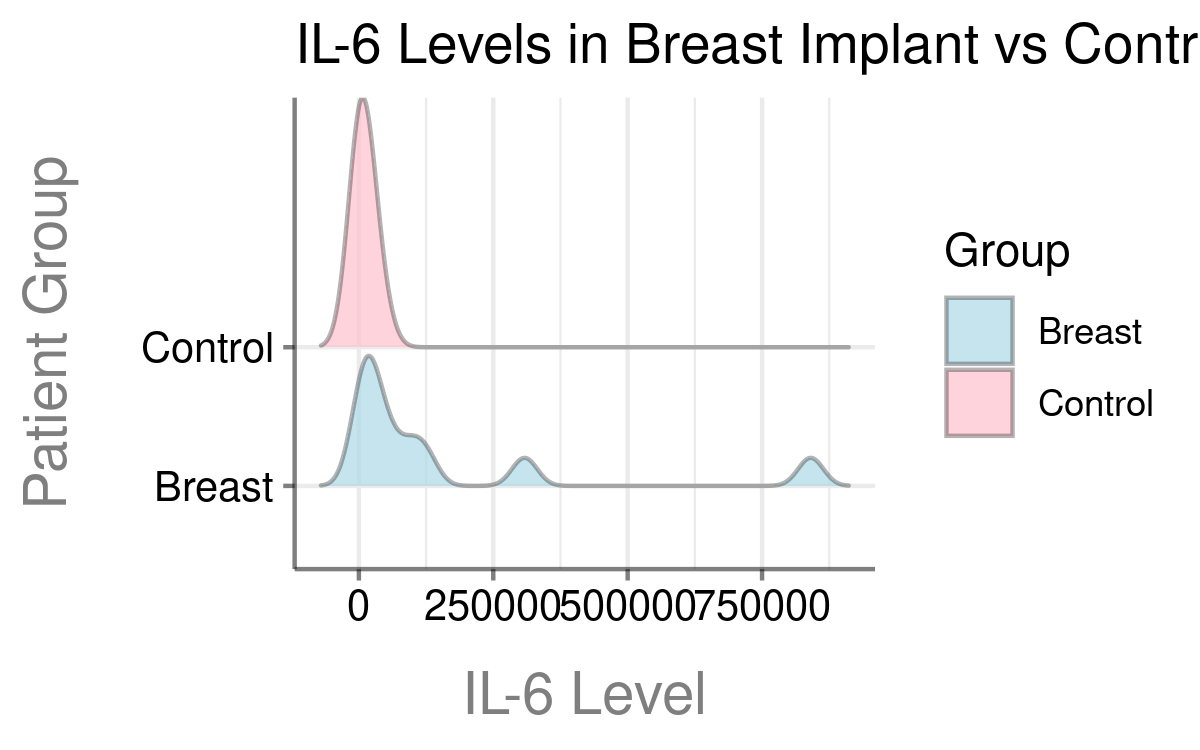
\includegraphics{DH302_Spring2025_Assignment02_files/figure-pdf/unnamed-chunk-7-1.png}

\paragraph{2b. Draw a Q-Q plot for both the measurements {[}5
points{]}}\label{b.-draw-a-q-q-plot-for-both-the-measurements-5-points}

You can use the
\href{https://ggplot2.tidyverse.org/reference/geom_qq.html}{geom\_qq}
function

\begin{Shaded}
\begin{Highlighting}[]
\CommentTok{\# YOUR CODE HERE FOR GENERATING A QQ PLOT}

\CommentTok{\# FIX ME {-} replace this with something that will give you a qqplot}
\NormalTok{implant.qqplot }\OtherTok{\textless{}{-}} \FunctionTok{ggplot}\NormalTok{(df.breast, }\FunctionTok{aes}\NormalTok{(}\AttributeTok{sample =}\NormalTok{ value)) }\SpecialCharTok{+}
  \FunctionTok{geom\_qq}\NormalTok{(}\AttributeTok{distribution =}\NormalTok{ stats}\SpecialCharTok{::}\NormalTok{qnorm, , }\AttributeTok{alpha=}\FloatTok{0.5}\NormalTok{) }\SpecialCharTok{+}
  \FunctionTok{geom\_qq\_line}\NormalTok{(}\AttributeTok{distribution =}\NormalTok{ stats}\SpecialCharTok{::}\NormalTok{qnorm, }\AttributeTok{alpha=}\FloatTok{0.3}\NormalTok{) }\SpecialCharTok{+}
  \FunctionTok{ggtitle}\NormalTok{(}\StringTok{"Breast Implant"}\NormalTok{) }\SpecialCharTok{+}
  \FunctionTok{theme\_minimal}\NormalTok{() }\SpecialCharTok{+}
\NormalTok{  theme}

\CommentTok{\# FIX ME  {-} replace this with something that will give you a qqplot}
\NormalTok{control.qqplot }\OtherTok{\textless{}{-}} \FunctionTok{ggplot}\NormalTok{(df.control, }\FunctionTok{aes}\NormalTok{(}\AttributeTok{sample =}\NormalTok{ value)) }\SpecialCharTok{+}
  \FunctionTok{geom\_qq}\NormalTok{(}\AttributeTok{distribution =}\NormalTok{ stats}\SpecialCharTok{::}\NormalTok{qnorm, }\AttributeTok{alpha=}\FloatTok{0.5}\NormalTok{) }\SpecialCharTok{+}
  \FunctionTok{geom\_qq\_line}\NormalTok{(}\AttributeTok{distribution =}\NormalTok{ stats}\SpecialCharTok{::}\NormalTok{qnorm, }\AttributeTok{alpha=}\FloatTok{0.3}\NormalTok{) }\SpecialCharTok{+}
  \FunctionTok{ggtitle}\NormalTok{(}\StringTok{"Control "}\NormalTok{) }\SpecialCharTok{+}
  \FunctionTok{theme\_minimal}\NormalTok{() }\SpecialCharTok{+}
\NormalTok{  theme}

\CommentTok{\# !! DO NOT EDIT/REMOVE !!}
\FunctionTok{library}\NormalTok{(patchwork)}
\NormalTok{implant.qqplot }\SpecialCharTok{|}\NormalTok{ control.qqplot}
\end{Highlighting}
\end{Shaded}

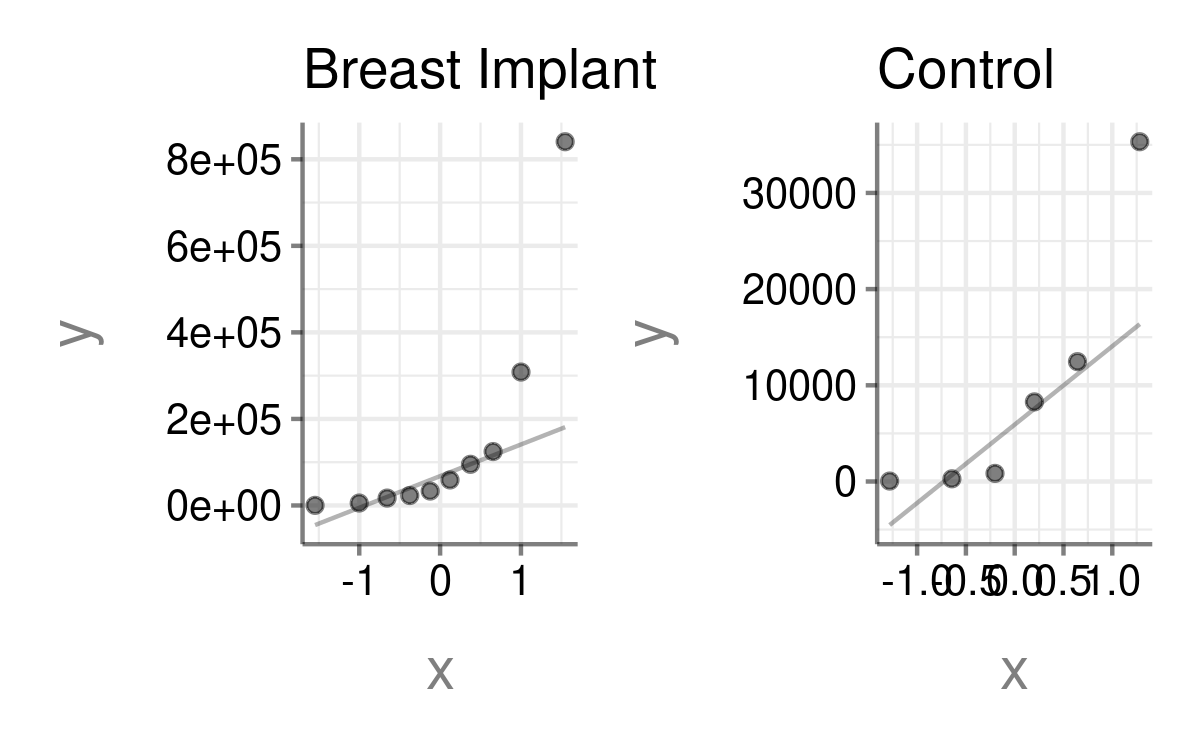
\includegraphics{DH302_Spring2025_Assignment02_files/figure-pdf/unnamed-chunk-8-1.png}

\section{Problem 03 {[}10 points{]}}\label{problem-03-10-points}

\textbf{Sneak peek:} I perform a t test of the null hypothesis that two
means are equal. I decided to calculate the means and then choose an
alternative hypothesis \(H_A\) \(\mu_1>\mu_2\) because I observed
\(\bar{y}_1 >\bar{y}_2\).

\paragraph{3a. Explain what is wrong (if anything) with this procedure
and why it is wrong (if anything). {[}5
points{]}}\label{a.-explain-what-is-wrong-if-anything-with-this-procedure-and-why-it-is-wrong-if-anything.-5-points}

\paragraph{\texorpdfstring{\textbf{Answer:}}{Answer:}}\label{answer}

We need to define the null and alternative hypothesis before performing
the tests. This is because looking at the data before can
unintentionally bias our hypothesis towards patterns observed in the
sample.

\paragraph{3b. Suppose I reported t = 1.97 on 25 degrees of freedom and
a P-value of 0.03. What is the proper P-value? {[}5
points{]}}\label{b.-suppose-i-reported-t-1.97-on-25-degrees-of-freedom-and-a-p-value-of-0.03.-what-is-the-proper-p-value-5-points}

\textbf{Answer:}

We should use a two-tailed test since alternative hypothesis was not
pre-specified. Hence the true \(p-value\) is \(2×p-value(T≥1.97)\) =
\(0.06\).

\section{Problem 04 {[}25 points{]}}\label{problem-04-25-points}

\textbf{``What I cannot build, I cannot understand -- Feynman''.} We
studied different t-tests and summarised it
\href{https://docs.google.com/presentation/d/15kxh03hVBR1ybnuBBvbT5pfInju1IVkmVH1trWbKJn4/edit\#slide=id.g32ec1a320fa_0_59}{here}.
This was like a recipe - do this when you have this ingredient, do that
if not. The goal of this problem is to flip this and figure out what
happens if we try breaking this assumption

\subsubsection{\texorpdfstring{4a. \textbf{The defaults}. Simulate two
normal samples (n=200) with each mean = 10 and sd = 1, 10000 times.
Apply a t-test for each iteration and calculate the p-value. With
\(\alpha=0.05\), how many times do you reject the null hypothesis that
the mean of two samples is equal? What do you conclude? {[}2.5
points{]}}{4a. The defaults. Simulate two normal samples (n=200) with each mean = 10 and sd = 1, 10000 times. Apply a t-test for each iteration and calculate the p-value. With \textbackslash alpha=0.05, how many times do you reject the null hypothesis that the mean of two samples is equal? What do you conclude? {[}2.5 points{]}}}\label{a.-the-defaults.-simulate-two-normal-samples-n200-with-each-mean-10-and-sd-1-10000-times.-apply-a-t-test-for-each-iteration-and-calculate-the-p-value.-with-alpha0.05-how-many-times-do-you-reject-the-null-hypothesis-that-the-mean-of-two-samples-is-equal-what-do-you-conclude-2.5-points}

\begin{Shaded}
\begin{Highlighting}[]
\CommentTok{\# \# !! DO NOT EDIT/REMOVE !!}
\CommentTok{\# OUTPUT: n\_rejects {-}{-} Number of rejections for alpha=0.05}

\FunctionTok{set.seed}\NormalTok{(}\DecValTok{42}\NormalTok{)}
\NormalTok{alpha }\OtherTok{\textless{}{-}} \FloatTok{0.05}
\NormalTok{n\_rejections }\OtherTok{\textless{}{-}} \DecValTok{0}
\NormalTok{N\_tries }\OtherTok{\textless{}{-}} \DecValTok{10000}
\NormalTok{n\_sample\_size }\OtherTok{\textless{}{-}} \DecValTok{200}

\ControlFlowTok{for}\NormalTok{ (i }\ControlFlowTok{in} \DecValTok{1} \SpecialCharTok{:}\NormalTok{ N\_tries) \{}
  
\NormalTok{  s1 }\OtherTok{\textless{}{-}} \FunctionTok{rnorm}\NormalTok{(n\_sample\_size, }\AttributeTok{mean =} \DecValTok{10}\NormalTok{, }\AttributeTok{sd =} \DecValTok{1}\NormalTok{)}
\NormalTok{  s2 }\OtherTok{\textless{}{-}} \FunctionTok{rnorm}\NormalTok{(n\_sample\_size, }\AttributeTok{mean =} \DecValTok{10}\NormalTok{, }\AttributeTok{sd =} \DecValTok{1}\NormalTok{)}
\NormalTok{  test\_stat }\OtherTok{\textless{}{-}} \FunctionTok{t.test}\NormalTok{(s1, s2)}
\NormalTok{  p\_value }\OtherTok{\textless{}{-}}\NormalTok{ test\_stat}\SpecialCharTok{$}\NormalTok{p.value}
  
  \ControlFlowTok{if}\NormalTok{ (p\_value }\SpecialCharTok{\textless{}}\NormalTok{ alpha) \{}
\NormalTok{    n\_rejections }\OtherTok{\textless{}{-}}\NormalTok{ n\_rejections }\SpecialCharTok{+} \DecValTok{1}
\NormalTok{  \}}
\NormalTok{\}}

\CommentTok{\# YOUR RESPONSE HERE}
\NormalTok{n\_rejections }\SpecialCharTok{/}\NormalTok{ N\_tries}
\end{Highlighting}
\end{Shaded}

\begin{verbatim}
[1] 0.0511
\end{verbatim}

\textbf{n\_rejections/N\_tries:} 0.0511

\textbf{Conclusion:} Since our significance level is 0.05, the
probability of getting null hypothesis rejected should be around 0.05
only. Our above experiment confirms it, the rate of rejection is indeed
close to 0.05.

\subsubsection{\texorpdfstring{4b. \textbf{Unequal variance}. Simulate
two normal samples (n=100) with each mean = 10 and sd1 = 1 and sd2=2.5,
10000 times. Apply a t-test for each iteration and calculate the
p-value. With \(\alpha=0.05\), how many times do you reject the null
hypothesis that the mean of two samples is equal? What do you conclude
and is that unusual? Use the default \texttt{t.test} {[}2.5
points{]}}{4b. Unequal variance. Simulate two normal samples (n=100) with each mean = 10 and sd1 = 1 and sd2=2.5, 10000 times. Apply a t-test for each iteration and calculate the p-value. With \textbackslash alpha=0.05, how many times do you reject the null hypothesis that the mean of two samples is equal? What do you conclude and is that unusual? Use the default t.test {[}2.5 points{]}}}\label{b.-unequal-variance.-simulate-two-normal-samples-n100-with-each-mean-10-and-sd1-1-and-sd22.5-10000-times.-apply-a-t-test-for-each-iteration-and-calculate-the-p-value.-with-alpha0.05-how-many-times-do-you-reject-the-null-hypothesis-that-the-mean-of-two-samples-is-equal-what-do-you-conclude-and-is-that-unusual-use-the-default-t.test-2.5-points}

\begin{Shaded}
\begin{Highlighting}[]
\CommentTok{\# OUTPUT: n\_rejects {-}{-} Number of rejections for alpha=0.05}

\FunctionTok{set.seed}\NormalTok{(}\DecValTok{42}\NormalTok{)}
\NormalTok{alpha }\OtherTok{\textless{}{-}} \FloatTok{0.05}
\NormalTok{n\_rejections }\OtherTok{\textless{}{-}} \DecValTok{0}
\NormalTok{N\_tries }\OtherTok{\textless{}{-}} \DecValTok{10000}
\NormalTok{n\_sample\_size }\OtherTok{\textless{}{-}} \DecValTok{200}
\NormalTok{mean1 }\OtherTok{\textless{}{-}} \DecValTok{10}
\NormalTok{mean2 }\OtherTok{\textless{}{-}}\NormalTok{ mean1}

\NormalTok{sd1 }\OtherTok{\textless{}{-}} \DecValTok{1}
\NormalTok{sd2 }\OtherTok{\textless{}{-}} \FloatTok{2.5}

\ControlFlowTok{for}\NormalTok{ (i }\ControlFlowTok{in} \DecValTok{1}\SpecialCharTok{:}\NormalTok{N\_tries) \{}
  
\NormalTok{  s1 }\OtherTok{\textless{}{-}} \FunctionTok{rnorm}\NormalTok{(n\_sample\_size, }\AttributeTok{mean =} \DecValTok{10}\NormalTok{, }\AttributeTok{sd =} \DecValTok{1}\NormalTok{)}
\NormalTok{  s2 }\OtherTok{\textless{}{-}} \FunctionTok{rnorm}\NormalTok{(n\_sample\_size, }\AttributeTok{mean =} \DecValTok{10}\NormalTok{, }\AttributeTok{sd =} \FloatTok{2.5}\NormalTok{)}
\NormalTok{  test\_stat }\OtherTok{\textless{}{-}} \FunctionTok{t.test}\NormalTok{(s1, s2)}
\NormalTok{  p\_value }\OtherTok{\textless{}{-}}\NormalTok{ test\_stat}\SpecialCharTok{$}\NormalTok{p.value}
  
  \ControlFlowTok{if}\NormalTok{ (p\_value }\SpecialCharTok{\textless{}}\NormalTok{ alpha) \{}
\NormalTok{    n\_rejections }\OtherTok{\textless{}{-}}\NormalTok{ n\_rejections }\SpecialCharTok{+} \DecValTok{1}
\NormalTok{  \}}
\NormalTok{\}}

\CommentTok{\# YOUR RESPONSE HERE}

\NormalTok{n\_rejections }\SpecialCharTok{/}\NormalTok{ N\_tries}
\end{Highlighting}
\end{Shaded}

\begin{verbatim}
[1] 0.0519
\end{verbatim}

\textbf{n\_rejections/N\_tries:} 0.0519

\textbf{Conclusion:} Even when we are not accounting for unequal
variances, we are getting correct rejection rate. The reason is that for
large and equal samples, Welch's test and the default t-test gives the
same result.

\subsubsection{\texorpdfstring{4c. \textbf{Unequal variance revisited}:
Repeat the example in 4b with now
\texttt{var.equal=FALSE}:\texttt{t.test(var.equal=TRUE)}. With
\(\alpha=0.05\), how many times do you reject the null hypothesis that
the mean of two samples is equal? What do you conclude? {[}2.5
points{]}}{4c. Unequal variance revisited: Repeat the example in 4b with now var.equal=FALSE:t.test(var.equal=TRUE). With \textbackslash alpha=0.05, how many times do you reject the null hypothesis that the mean of two samples is equal? What do you conclude? {[}2.5 points{]}}}\label{c.-unequal-variance-revisited-repeat-the-example-in-4b-with-now-var.equalfalset.testvar.equaltrue.-with-alpha0.05-how-many-times-do-you-reject-the-null-hypothesis-that-the-mean-of-two-samples-is-equal-what-do-you-conclude-2.5-points}

\begin{Shaded}
\begin{Highlighting}[]
\CommentTok{\# OUTPUT: n\_rejects {-}{-} Number of rejections for alpha=0.05}

\FunctionTok{set.seed}\NormalTok{(}\DecValTok{42}\NormalTok{)}
\NormalTok{alpha }\OtherTok{\textless{}{-}} \FloatTok{0.05}
\NormalTok{n\_rejections }\OtherTok{\textless{}{-}} \DecValTok{0}
\NormalTok{N\_tries }\OtherTok{\textless{}{-}} \DecValTok{10000}
\NormalTok{n\_sample\_size }\OtherTok{\textless{}{-}} \DecValTok{200}
\NormalTok{mean1 }\OtherTok{\textless{}{-}} \DecValTok{10}
\NormalTok{mean2 }\OtherTok{\textless{}{-}}\NormalTok{ mean1}

\NormalTok{sd1 }\OtherTok{\textless{}{-}} \DecValTok{1}
\NormalTok{sd2 }\OtherTok{\textless{}{-}} \FloatTok{2.5}

\ControlFlowTok{for}\NormalTok{ (i }\ControlFlowTok{in} \DecValTok{1}\SpecialCharTok{:}\NormalTok{N\_tries) \{}
  
\NormalTok{  s1 }\OtherTok{\textless{}{-}} \FunctionTok{rnorm}\NormalTok{(n\_sample\_size, }\AttributeTok{mean =} \DecValTok{10}\NormalTok{, }\AttributeTok{sd =} \DecValTok{1}\NormalTok{)}
\NormalTok{  s2 }\OtherTok{\textless{}{-}} \FunctionTok{rnorm}\NormalTok{(n\_sample\_size, }\AttributeTok{mean =} \DecValTok{10}\NormalTok{, }\AttributeTok{sd =} \FloatTok{2.5}\NormalTok{)}
\NormalTok{  test\_stat }\OtherTok{\textless{}{-}} \FunctionTok{t.test}\NormalTok{(s1, s2, }\AttributeTok{var.equal =} \ConstantTok{FALSE}\NormalTok{)}
\NormalTok{  p\_value }\OtherTok{\textless{}{-}}\NormalTok{ test\_stat}\SpecialCharTok{$}\NormalTok{p.value}
  
  \ControlFlowTok{if}\NormalTok{ (p\_value }\SpecialCharTok{\textless{}}\NormalTok{ alpha) \{}
\NormalTok{    n\_rejections }\OtherTok{\textless{}{-}}\NormalTok{ n\_rejections }\SpecialCharTok{+} \DecValTok{1}
\NormalTok{  \}}
\NormalTok{\}}

\CommentTok{\# YOUR RESPONSE HERE}
\NormalTok{n\_rejections }\SpecialCharTok{/}\NormalTok{ N\_tries}
\end{Highlighting}
\end{Shaded}

\begin{verbatim}
[1] 0.0519
\end{verbatim}

\textbf{n\_rejections/N\_tries:} 0.0519

\textbf{Conclusion:} Our observations are correct since Welch's test
accounts for difference in variances.

\paragraph{\texorpdfstring{4d. \textbf{Severe violation}: Following 4c,
now set sd1=10, sd2=1, and use a non-welch t-test to tabulate the number
of times you reject the null? With \(\alpha=0.05\), how many times do
you reject the null hypothesis that the mean of two samples is equal?
What do you conclude? {[}2.5
points{]}}{4d. Severe violation: Following 4c, now set sd1=10, sd2=1, and use a non-welch t-test to tabulate the number of times you reject the null? With \textbackslash alpha=0.05, how many times do you reject the null hypothesis that the mean of two samples is equal? What do you conclude? {[}2.5 points{]}}}\label{d.-severe-violation-following-4c-now-set-sd110-sd21-and-use-a-non-welch-t-test-to-tabulate-the-number-of-times-you-reject-the-null-with-alpha0.05-how-many-times-do-you-reject-the-null-hypothesis-that-the-mean-of-two-samples-is-equal-what-do-you-conclude-2.5-points}

\begin{Shaded}
\begin{Highlighting}[]
\CommentTok{\# OUTPUT: n\_rejects {-}{-} Number of rejections for alpha=0.05}

\FunctionTok{set.seed}\NormalTok{(}\DecValTok{42}\NormalTok{)}
\NormalTok{alpha }\OtherTok{\textless{}{-}} \FloatTok{0.05}
\NormalTok{n\_rejections }\OtherTok{\textless{}{-}} \DecValTok{0}
\NormalTok{N\_tries }\OtherTok{\textless{}{-}} \DecValTok{10000}
\NormalTok{n\_sample\_size }\OtherTok{\textless{}{-}} \DecValTok{200}

\NormalTok{mean1 }\OtherTok{\textless{}{-}} \DecValTok{10}
\NormalTok{mean2 }\OtherTok{\textless{}{-}}\NormalTok{ mean1}

\NormalTok{sd1 }\OtherTok{\textless{}{-}} \DecValTok{10}
\NormalTok{sd2 }\OtherTok{\textless{}{-}} \DecValTok{1}

\ControlFlowTok{for}\NormalTok{ (i }\ControlFlowTok{in} \DecValTok{1}\SpecialCharTok{:}\NormalTok{N\_tries) \{}
  
\NormalTok{  s1 }\OtherTok{\textless{}{-}} \FunctionTok{rnorm}\NormalTok{(n\_sample\_size, }\AttributeTok{mean =} \DecValTok{10}\NormalTok{, }\AttributeTok{sd =} \DecValTok{1}\NormalTok{)}
\NormalTok{  s2 }\OtherTok{\textless{}{-}} \FunctionTok{rnorm}\NormalTok{(n\_sample\_size, }\AttributeTok{mean =} \DecValTok{10}\NormalTok{, }\AttributeTok{sd =} \FloatTok{2.5}\NormalTok{)}
\NormalTok{  test\_stat }\OtherTok{\textless{}{-}} \FunctionTok{t.test}\NormalTok{(s1, s2, }\AttributeTok{var.equal =} \ConstantTok{TRUE}\NormalTok{)}
\NormalTok{  p\_value }\OtherTok{\textless{}{-}}\NormalTok{ test\_stat}\SpecialCharTok{$}\NormalTok{p.value}
  
  \ControlFlowTok{if}\NormalTok{ (p\_value }\SpecialCharTok{\textless{}}\NormalTok{ alpha) \{}
\NormalTok{    n\_rejections }\OtherTok{\textless{}{-}}\NormalTok{ n\_rejections }\SpecialCharTok{+} \DecValTok{1}
\NormalTok{  \}}
\NormalTok{\}}

\CommentTok{\# YOUR RESPONSE HERE}

\NormalTok{n\_rejections }\SpecialCharTok{/}\NormalTok{ N\_tries}
\end{Highlighting}
\end{Shaded}

\begin{verbatim}
[1] 0.0523
\end{verbatim}

\textbf{n\_rejections/N\_tries:} 0.0523

\textbf{Conclusion:} Since the variances differ a lot, and the test we
are doing here does not account for variance differences, we see a
higher rejection rate of null hypothesis compared to \(\alpha\).

\paragraph{\texorpdfstring{4e. \textbf{Severe violation2}: Following 4d,
now simulate different sample sizes with n\_sample\_size1 =30 and
n\_sample\_size2=70, sd1=10, sd2=1, and use a non=welch t-test to
tabulate the number of times you reject the null? With \(\alpha=0.05\),
how many times do you reject the null hypothesis that the mean of two
samples is equal? What do you conclude? {[}2.5
points{]}}{4e. Severe violation2: Following 4d, now simulate different sample sizes with n\_sample\_size1 =30 and n\_sample\_size2=70, sd1=10, sd2=1, and use a non=welch t-test to tabulate the number of times you reject the null? With \textbackslash alpha=0.05, how many times do you reject the null hypothesis that the mean of two samples is equal? What do you conclude? {[}2.5 points{]}}}\label{e.-severe-violation2-following-4d-now-simulate-different-sample-sizes-with-n_sample_size1-30-and-n_sample_size270-sd110-sd21-and-use-a-nonwelch-t-test-to-tabulate-the-number-of-times-you-reject-the-null-with-alpha0.05-how-many-times-do-you-reject-the-null-hypothesis-that-the-mean-of-two-samples-is-equal-what-do-you-conclude-2.5-points}

\begin{Shaded}
\begin{Highlighting}[]
\CommentTok{\# OUTPUT: n\_rejects {-}{-} Number of rejections for alpha=0.05}

\FunctionTok{set.seed}\NormalTok{(}\DecValTok{42}\NormalTok{)}
\NormalTok{alpha }\OtherTok{\textless{}{-}} \FloatTok{0.05}
\NormalTok{n\_rejections }\OtherTok{\textless{}{-}} \DecValTok{0}
\NormalTok{N\_tries }\OtherTok{\textless{}{-}} \DecValTok{10000}
\NormalTok{n\_sample\_size1 }\OtherTok{\textless{}{-}} \DecValTok{30}
\NormalTok{n\_sample\_size2 }\OtherTok{\textless{}{-}} \DecValTok{70}
\NormalTok{mean1 }\OtherTok{\textless{}{-}} \DecValTok{10}
\NormalTok{mean2 }\OtherTok{\textless{}{-}}\NormalTok{ mean1}

\NormalTok{sd1 }\OtherTok{\textless{}{-}} \DecValTok{10}
\NormalTok{sd2 }\OtherTok{\textless{}{-}} \DecValTok{1}

\ControlFlowTok{for}\NormalTok{ (i }\ControlFlowTok{in} \DecValTok{1}\SpecialCharTok{:}\NormalTok{N\_tries) \{}
  
\NormalTok{  s1 }\OtherTok{\textless{}{-}} \FunctionTok{rnorm}\NormalTok{(n\_sample\_size1, }\AttributeTok{mean =}\NormalTok{ mean1, }\AttributeTok{sd =}\NormalTok{ sd1)}
\NormalTok{  s2 }\OtherTok{\textless{}{-}} \FunctionTok{rnorm}\NormalTok{(n\_sample\_size2, }\AttributeTok{mean =}\NormalTok{ mean2, }\AttributeTok{sd =}\NormalTok{ sd2)}
\NormalTok{  test\_stat }\OtherTok{\textless{}{-}} \FunctionTok{t.test}\NormalTok{(s1, s2, }\AttributeTok{var.equal =} \ConstantTok{TRUE}\NormalTok{)}
\NormalTok{  p\_value }\OtherTok{\textless{}{-}}\NormalTok{ test\_stat}\SpecialCharTok{$}\NormalTok{p.value}
  
  \ControlFlowTok{if}\NormalTok{ (p\_value }\SpecialCharTok{\textless{}}\NormalTok{ alpha) \{}
\NormalTok{    n\_rejections }\OtherTok{\textless{}{-}}\NormalTok{ n\_rejections }\SpecialCharTok{+} \DecValTok{1}
\NormalTok{  \}}
\NormalTok{\}}

\CommentTok{\# YOUR RESPONSE HERE}
\NormalTok{n\_rejections }\SpecialCharTok{/}\NormalTok{ N\_tries}
\end{Highlighting}
\end{Shaded}

\begin{verbatim}
[1] 0.2068
\end{verbatim}

\textbf{n\_rejections/N\_tries:} 0.2068

\textbf{Conclusion:} Here we have both unequal sized samples and unequal
variances. Using a default t-test gives us an unusually high rejection
rate, around 0.2. The default t-test fails badly on data with unequal
means and variances.

\paragraph{\texorpdfstring{4f. \textbf{Severe violation3}: Repeat 4e
with n\_sample\_size1 = 70 and n\_sample\_size2=30, sd1=10, sd2=1, and
use a non-welch t-test to tabulate the number of times you reject the
null? With \(\alpha=0.05\), how many times do you reject the null
hypothesis that the mean of two samples is equal? What do you conclude?
{[}2.5
points{]}}{4f. Severe violation3: Repeat 4e with n\_sample\_size1 = 70 and n\_sample\_size2=30, sd1=10, sd2=1, and use a non-welch t-test to tabulate the number of times you reject the null? With \textbackslash alpha=0.05, how many times do you reject the null hypothesis that the mean of two samples is equal? What do you conclude? {[}2.5 points{]}}}\label{f.-severe-violation3-repeat-4e-with-n_sample_size1-70-and-n_sample_size230-sd110-sd21-and-use-a-non-welch-t-test-to-tabulate-the-number-of-times-you-reject-the-null-with-alpha0.05-how-many-times-do-you-reject-the-null-hypothesis-that-the-mean-of-two-samples-is-equal-what-do-you-conclude-2.5-points}

\begin{Shaded}
\begin{Highlighting}[]
\CommentTok{\# OUTPUT: n\_rejects {-}{-} Number of rejections for alpha=0.05}

\FunctionTok{set.seed}\NormalTok{(}\DecValTok{42}\NormalTok{)}
\NormalTok{alpha }\OtherTok{\textless{}{-}} \FloatTok{0.05}
\NormalTok{n\_rejections }\OtherTok{\textless{}{-}} \DecValTok{0}
\NormalTok{N\_tries }\OtherTok{\textless{}{-}} \DecValTok{10000}
\NormalTok{n\_sample\_size1 }\OtherTok{\textless{}{-}} \DecValTok{70}
\NormalTok{n\_sample\_size2 }\OtherTok{\textless{}{-}} \DecValTok{30}
\NormalTok{mean1 }\OtherTok{\textless{}{-}} \DecValTok{10}
\NormalTok{mean2 }\OtherTok{\textless{}{-}}\NormalTok{ mean1}

\NormalTok{sd1 }\OtherTok{\textless{}{-}} \DecValTok{10}
\NormalTok{sd2 }\OtherTok{\textless{}{-}} \DecValTok{1}

\ControlFlowTok{for}\NormalTok{ (i }\ControlFlowTok{in} \DecValTok{1}\SpecialCharTok{:}\NormalTok{N\_tries) \{}
  
\NormalTok{  s1 }\OtherTok{\textless{}{-}} \FunctionTok{rnorm}\NormalTok{(n\_sample\_size1, }\AttributeTok{mean =}\NormalTok{ mean1, }\AttributeTok{sd =}\NormalTok{ sd1)}
\NormalTok{  s2 }\OtherTok{\textless{}{-}} \FunctionTok{rnorm}\NormalTok{(n\_sample\_size2, }\AttributeTok{mean =}\NormalTok{ mean2, }\AttributeTok{sd =}\NormalTok{ sd2)}
\NormalTok{  test\_stat }\OtherTok{\textless{}{-}} \FunctionTok{t.test}\NormalTok{(s1, s2, }\AttributeTok{var.equal =} \ConstantTok{TRUE}\NormalTok{)}
\NormalTok{  p\_value }\OtherTok{\textless{}{-}}\NormalTok{ test\_stat}\SpecialCharTok{$}\NormalTok{p.value}
  
  \ControlFlowTok{if}\NormalTok{ (p\_value }\SpecialCharTok{\textless{}}\NormalTok{ alpha) \{}
\NormalTok{    n\_rejections }\OtherTok{\textless{}{-}}\NormalTok{ n\_rejections }\SpecialCharTok{+} \DecValTok{1}
\NormalTok{  \}}
\NormalTok{\}}

\CommentTok{\# YOUR RESPONSE HERE}
\NormalTok{n\_rejections }\SpecialCharTok{/}\NormalTok{ N\_tries}
\end{Highlighting}
\end{Shaded}

\begin{verbatim}
[1] 0.0043
\end{verbatim}

\textbf{n\_rejections/N\_tries:} 0.0043

\textbf{Conclusion:} Which group (larger or smaller) has what variance
(larger or smaller) is deciding the rejection rate. But in any case, the
non-Welch t-test is failing and giving us wrong results.

\paragraph{\texorpdfstring{4g. \textbf{Severe violation4}: Repeat 4f
with n\_sample\_size1 = 70 and n\_sample\_size1=70, sd1=10, sd2=1, and
use a Welch t-test to tabulate the number of times you reject the null?
With \(\alpha=0.05\), how many times do you reject the null hypothesis
that the mean of two samples is equal? What do you conclude? {[}2.5
points{]}}{4g. Severe violation4: Repeat 4f with n\_sample\_size1 = 70 and n\_sample\_size1=70, sd1=10, sd2=1, and use a Welch t-test to tabulate the number of times you reject the null? With \textbackslash alpha=0.05, how many times do you reject the null hypothesis that the mean of two samples is equal? What do you conclude? {[}2.5 points{]}}}\label{g.-severe-violation4-repeat-4f-with-n_sample_size1-70-and-n_sample_size170-sd110-sd21-and-use-a-welch-t-test-to-tabulate-the-number-of-times-you-reject-the-null-with-alpha0.05-how-many-times-do-you-reject-the-null-hypothesis-that-the-mean-of-two-samples-is-equal-what-do-you-conclude-2.5-points}

\begin{Shaded}
\begin{Highlighting}[]
\CommentTok{\# OUTPUT: n\_rejects {-}{-} Number of rejections for alpha=0.05}

\FunctionTok{set.seed}\NormalTok{(}\DecValTok{42}\NormalTok{)}
\NormalTok{alpha }\OtherTok{\textless{}{-}} \FloatTok{0.05}
\NormalTok{n\_rejections }\OtherTok{\textless{}{-}} \DecValTok{0}
\NormalTok{N\_tries }\OtherTok{\textless{}{-}} \DecValTok{10000}
\NormalTok{n\_sample\_size1 }\OtherTok{\textless{}{-}} \DecValTok{70}
\NormalTok{n\_sample\_size2 }\OtherTok{\textless{}{-}} \DecValTok{30}
\NormalTok{mean1 }\OtherTok{\textless{}{-}} \DecValTok{10}
\NormalTok{mean2 }\OtherTok{\textless{}{-}}\NormalTok{ mean1}

\NormalTok{sd1 }\OtherTok{\textless{}{-}} \DecValTok{10}
\NormalTok{sd2 }\OtherTok{\textless{}{-}} \DecValTok{1}

\ControlFlowTok{for}\NormalTok{ (i }\ControlFlowTok{in} \DecValTok{1}\SpecialCharTok{:}\NormalTok{N\_tries) \{}
  
\NormalTok{  s1 }\OtherTok{\textless{}{-}} \FunctionTok{rnorm}\NormalTok{(n\_sample\_size1, }\AttributeTok{mean =}\NormalTok{ mean1, }\AttributeTok{sd =}\NormalTok{ sd1)}
\NormalTok{  s2 }\OtherTok{\textless{}{-}} \FunctionTok{rnorm}\NormalTok{(n\_sample\_size2, }\AttributeTok{mean =}\NormalTok{ mean2, }\AttributeTok{sd =}\NormalTok{ sd2)}
\NormalTok{  test\_stat }\OtherTok{\textless{}{-}} \FunctionTok{t.test}\NormalTok{(s1, s2, }\AttributeTok{var.equal =} \ConstantTok{TRUE}\NormalTok{)}
\NormalTok{  p\_value }\OtherTok{\textless{}{-}}\NormalTok{ test\_stat}\SpecialCharTok{$}\NormalTok{p.value}
  
  \ControlFlowTok{if}\NormalTok{ (p\_value }\SpecialCharTok{\textless{}}\NormalTok{ alpha) \{}
\NormalTok{    n\_rejections }\OtherTok{\textless{}{-}}\NormalTok{ n\_rejections }\SpecialCharTok{+} \DecValTok{1}
\NormalTok{  \}}
\NormalTok{\}}

\CommentTok{\# YOUR RESPONSE HERE}
\NormalTok{n\_rejections }\SpecialCharTok{/}\NormalTok{ N\_tries}
\end{Highlighting}
\end{Shaded}

\begin{verbatim}
[1] 0.0043
\end{verbatim}

\textbf{n\_rejections/N\_tries:} 0.0043

\textbf{Conclusion:} Which group (larger or smaller) has what variance
(larger or smaller) is deciding the rejection rate. But in any case, the
non-Welch t-test is failing and giving us wrong results.

\paragraph{\texorpdfstring{4h. \textbf{Toss in exponential}: Hopefully
you have got a feeling of what is happening. Now we take normality for a
toss. I have mentioned multiple times in the class, it is a relaxable
assumption, but is it really? {[}2.5
points{]}}{4h. Toss in exponential: Hopefully you have got a feeling of what is happening. Now we take normality for a toss. I have mentioned multiple times in the class, it is a relaxable assumption, but is it really? {[}2.5 points{]}}}\label{h.-toss-in-exponential-hopefully-you-have-got-a-feeling-of-what-is-happening.-now-we-take-normality-for-a-toss.-i-have-mentioned-multiple-times-in-the-class-it-is-a-relaxable-assumption-but-is-it-really-2.5-points}

For example if we simulate an exponential distribution this is what it
looks like

\begin{Shaded}
\begin{Highlighting}[]
\FunctionTok{set.seed}\NormalTok{(}\DecValTok{42}\NormalTok{)}

\NormalTok{exp\_data }\OtherTok{\textless{}{-}} \FunctionTok{rexp}\NormalTok{(}\DecValTok{100}\NormalTok{, }\AttributeTok{rate =} \DecValTok{5}\NormalTok{)}
\FunctionTok{qqnorm}\NormalTok{(exp\_data)}
\FunctionTok{qqline}\NormalTok{(exp\_data)}
\end{Highlighting}
\end{Shaded}

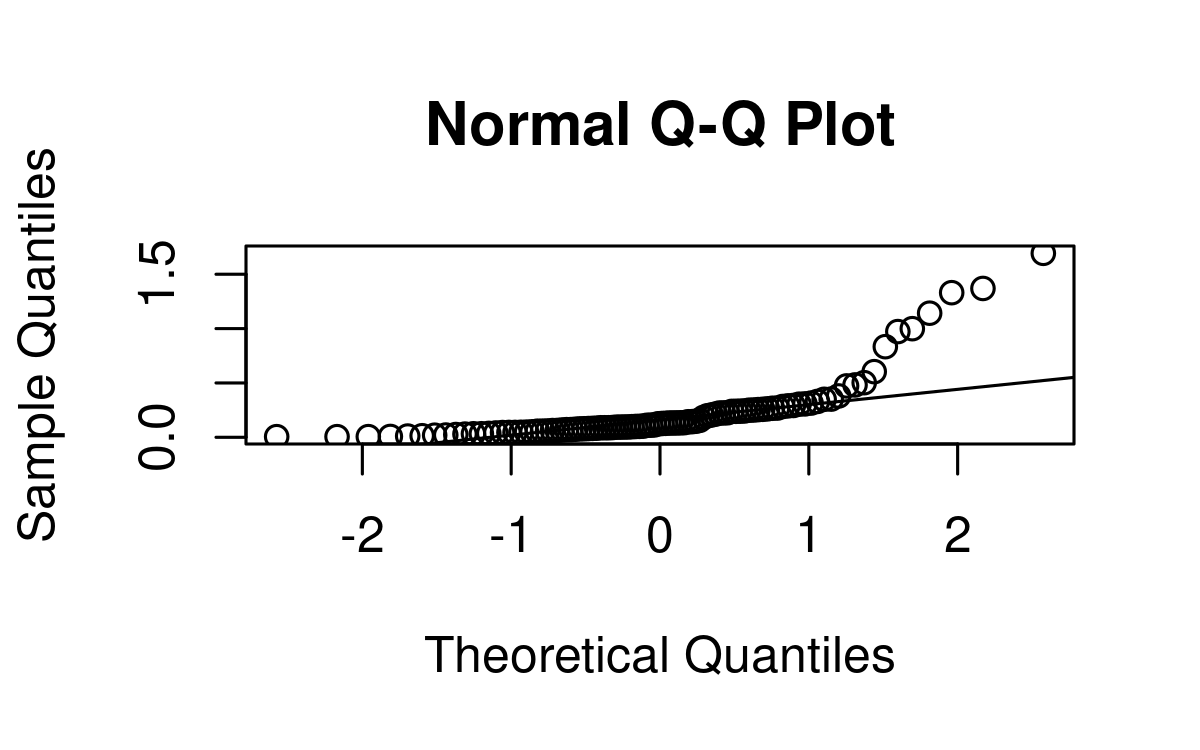
\includegraphics{DH302_Spring2025_Assignment02_files/figure-pdf/unnamed-chunk-16-1.png}

For a n\_sample\_size1 = 70 and n\_sample\_size1=n\_sample\_size2=100,
rate parameters r1=5 and r2=5 use a t-test to tabulate the number of
times you reject the null? With \(\alpha=0.05\), how many times do you
reject the null hypothesis that the mean of two samples is equal? What
do you conclude?

\begin{Shaded}
\begin{Highlighting}[]
\CommentTok{\# OUTPUT: n\_rejects {-}{-} Number of rejections for alpha=0.05}

\FunctionTok{set.seed}\NormalTok{(}\DecValTok{42}\NormalTok{)}
\NormalTok{alpha }\OtherTok{\textless{}{-}} \FloatTok{0.05}
\NormalTok{n\_rejections }\OtherTok{\textless{}{-}} \DecValTok{0}
\NormalTok{N\_tries }\OtherTok{\textless{}{-}} \DecValTok{10000}
\NormalTok{n\_sample\_size1 }\OtherTok{\textless{}{-}} \DecValTok{70}
\NormalTok{n\_sample\_size2 }\OtherTok{\textless{}{-}} \DecValTok{100}
\NormalTok{rate1 }\OtherTok{\textless{}{-}} \DecValTok{5}
\NormalTok{rate2 }\OtherTok{\textless{}{-}} \DecValTok{5}

\ControlFlowTok{for}\NormalTok{ (i }\ControlFlowTok{in} \DecValTok{1}\SpecialCharTok{:}\NormalTok{N\_tries) \{}
\NormalTok{  s1 }\OtherTok{\textless{}{-}} \FunctionTok{rexp}\NormalTok{(n\_sample\_size1, }\AttributeTok{rate =}\NormalTok{ rate1)}
\NormalTok{  s2 }\OtherTok{\textless{}{-}} \FunctionTok{rexp}\NormalTok{(n\_sample\_size2, }\AttributeTok{rate =}\NormalTok{ rate2)}
\NormalTok{  p\_value }\OtherTok{\textless{}{-}} \FunctionTok{t.test}\NormalTok{(s1, s2)}\SpecialCharTok{$}\NormalTok{p.value}
  \ControlFlowTok{if}\NormalTok{ (p\_value }\SpecialCharTok{\textless{}}\NormalTok{ alpha) \{}
\NormalTok{    n\_rejections }\OtherTok{\textless{}{-}}\NormalTok{ n\_rejections }\SpecialCharTok{+} \DecValTok{1}
\NormalTok{  \}}
\NormalTok{\}}


\CommentTok{\# YOUR RESPONSE HERE}

\NormalTok{n\_rejections }\SpecialCharTok{/}\NormalTok{ N\_tries}
\end{Highlighting}
\end{Shaded}

\begin{verbatim}
[1] 0.0511
\end{verbatim}

\textbf{n\_rejections/N\_tries:} 0.0511

\textbf{Conclusion:} Normality is indeed a relaxable condition, the
rejection rate we get is still close to 0.05. t-test is robust to
normality, given the sample sizes are sufficiently large.

\paragraph{\texorpdfstring{4i. \textbf{Toss in exponential2}: Following
4h, repeat the experment with sample\_size1=n\_sample\_size2=100, rate
parameters r1=5 and r2=10 use a t-test to tabulate the number of times
you reject the null? With \(\alpha=0.05\), how many times do you reject
the null hypothesis that the mean of two samples is equal? What do you
conclude? {[}5
points{]}}{4i. Toss in exponential2: Following 4h, repeat the experment with sample\_size1=n\_sample\_size2=100, rate parameters r1=5 and r2=10 use a t-test to tabulate the number of times you reject the null? With \textbackslash alpha=0.05, how many times do you reject the null hypothesis that the mean of two samples is equal? What do you conclude? {[}5 points{]}}}\label{i.-toss-in-exponential2-following-4h-repeat-the-experment-with-sample_size1n_sample_size2100-rate-parameters-r15-and-r210-use-a-t-test-to-tabulate-the-number-of-times-you-reject-the-null-with-alpha0.05-how-many-times-do-you-reject-the-null-hypothesis-that-the-mean-of-two-samples-is-equal-what-do-you-conclude-5-points}

\begin{Shaded}
\begin{Highlighting}[]
\CommentTok{\# OUTPUT: n\_rejects {-}{-} Number of rejections for alpha=0.05}

\FunctionTok{set.seed}\NormalTok{(}\DecValTok{42}\NormalTok{)}
\NormalTok{alpha }\OtherTok{\textless{}{-}} \FloatTok{0.05}
\NormalTok{n\_rejections }\OtherTok{\textless{}{-}} \DecValTok{0}
\NormalTok{N\_tries }\OtherTok{\textless{}{-}} \DecValTok{10000}
\NormalTok{n\_sample\_size1 }\OtherTok{\textless{}{-}} \DecValTok{100}
\NormalTok{n\_sample\_size2 }\OtherTok{\textless{}{-}} \DecValTok{100}
\NormalTok{rate1 }\OtherTok{\textless{}{-}} \DecValTok{5}
\NormalTok{rate2 }\OtherTok{\textless{}{-}} \DecValTok{10}

\ControlFlowTok{for}\NormalTok{ (i }\ControlFlowTok{in} \DecValTok{1}\SpecialCharTok{:}\NormalTok{N\_tries) \{}
\NormalTok{  s1 }\OtherTok{\textless{}{-}} \FunctionTok{rexp}\NormalTok{(n\_sample\_size1, }\AttributeTok{rate =}\NormalTok{ rate1)}
\NormalTok{  s2 }\OtherTok{\textless{}{-}} \FunctionTok{rexp}\NormalTok{(n\_sample\_size2, }\AttributeTok{rate =}\NormalTok{ rate2)}
\NormalTok{  p\_value }\OtherTok{\textless{}{-}} \FunctionTok{t.test}\NormalTok{(s1, s2)}\SpecialCharTok{$}\NormalTok{p.value}
  \ControlFlowTok{if}\NormalTok{ (p\_value }\SpecialCharTok{\textless{}}\NormalTok{ alpha) \{}
\NormalTok{    n\_rejections }\OtherTok{\textless{}{-}}\NormalTok{ n\_rejections }\SpecialCharTok{+} \DecValTok{1}
\NormalTok{  \}}
\NormalTok{\}}

\CommentTok{\# YOUR RESPONSE HERE}
\NormalTok{n\_rejections }\SpecialCharTok{/}\NormalTok{ N\_tries}
\end{Highlighting}
\end{Shaded}

\begin{verbatim}
[1] 0.9982
\end{verbatim}

\textbf{Conclusion:} This time the means are different, so we see a very
high rejection rate. This means that although the data is not normally
distributed, t-test works very well on it.

\section{Problem 05 {[}30 points{]}}\label{problem-05-30-points}

\textbf{Standard error:} Adults who broke their wrists were tested to
see if their grip strength (kg) decreased over 6 weeks. The data is
provided as a tsv
\href{https://drive.google.com/file/d/1HfzOESwZBuqNgEHX18Dfd4I7vTSwQOPh/view?usp=sharing}{here}.

\paragraph{5a. What is the null and alternative hypothesis? {[}2.5
points{]}}\label{a.-what-is-the-null-and-alternative-hypothesis-2.5-points}

\textbf{Answer:}

\(H_0\): There is no difference in the grip strengths of adults after 6
weeks.

\(H_A\): The grip strength of adults decreased during the period of 6
weeks.

\paragraph{5b. Which test would you employ to test your hypothesis and
why? {[}2.5
points{]}}\label{b.-which-test-would-you-employ-to-test-your-hypothesis-and-why-2.5-points}

\textbf{Answer:}

We use a paired t-test because it compares the same subjects before and
after 6 weeks. It is not a two group situation, we only have a single
group and we are observing it at different times and want to comment on
mean difference.

\paragraph{5c. If there are conditions to be satisfied for applying your
test, write R code to output checks for validity of your test. {[}5
points{]}}\label{c.-if-there-are-conditions-to-be-satisfied-for-applying-your-test-write-r-code-to-output-checks-for-validity-of-your-test.-5-points}

\begin{Shaded}
\begin{Highlighting}[]
\CommentTok{\# Load necessary library}
\FunctionTok{library}\NormalTok{(ggplot2)}

\NormalTok{data }\OtherTok{\textless{}{-}} \FunctionTok{read.delim}\NormalTok{(}\StringTok{"./Assignment02\_grip\_strength.tsv"}\NormalTok{)}

\CommentTok{\# difference in means}
\NormalTok{data}\SpecialCharTok{$}\NormalTok{diff }\OtherTok{\textless{}{-}}\NormalTok{ data}\SpecialCharTok{$}\NormalTok{baseline }\SpecialCharTok{{-}}\NormalTok{ data}\SpecialCharTok{$}\NormalTok{measured\_6weekslater}

\CommentTok{\# visualizing if the distribution of weight differences is normal}
\FunctionTok{ggplot}\NormalTok{(data, }\FunctionTok{aes}\NormalTok{(}\AttributeTok{x =}\NormalTok{ diff)) }\SpecialCharTok{+}
  \FunctionTok{geom\_histogram}\NormalTok{(}\AttributeTok{binwidth =} \DecValTok{2}\NormalTok{, }\AttributeTok{fill =} \StringTok{"lightblue"}\NormalTok{, }
                 \AttributeTok{color =}\NormalTok{ scales}\SpecialCharTok{::}\FunctionTok{alpha}\NormalTok{(}\StringTok{"black"}\NormalTok{, }\FloatTok{0.5}\NormalTok{)) }\SpecialCharTok{+}
  \FunctionTok{ggtitle}\NormalTok{(}\StringTok{"Histogram of Differences"}\NormalTok{) }\SpecialCharTok{+}
  \FunctionTok{xlab}\NormalTok{(}\StringTok{"Difference (Baseline {-} 6 Weeks)"}\NormalTok{) }\SpecialCharTok{+}
  \FunctionTok{ylab}\NormalTok{(}\StringTok{"Frequency"}\NormalTok{) }\SpecialCharTok{+}
\NormalTok{  theme}
\end{Highlighting}
\end{Shaded}

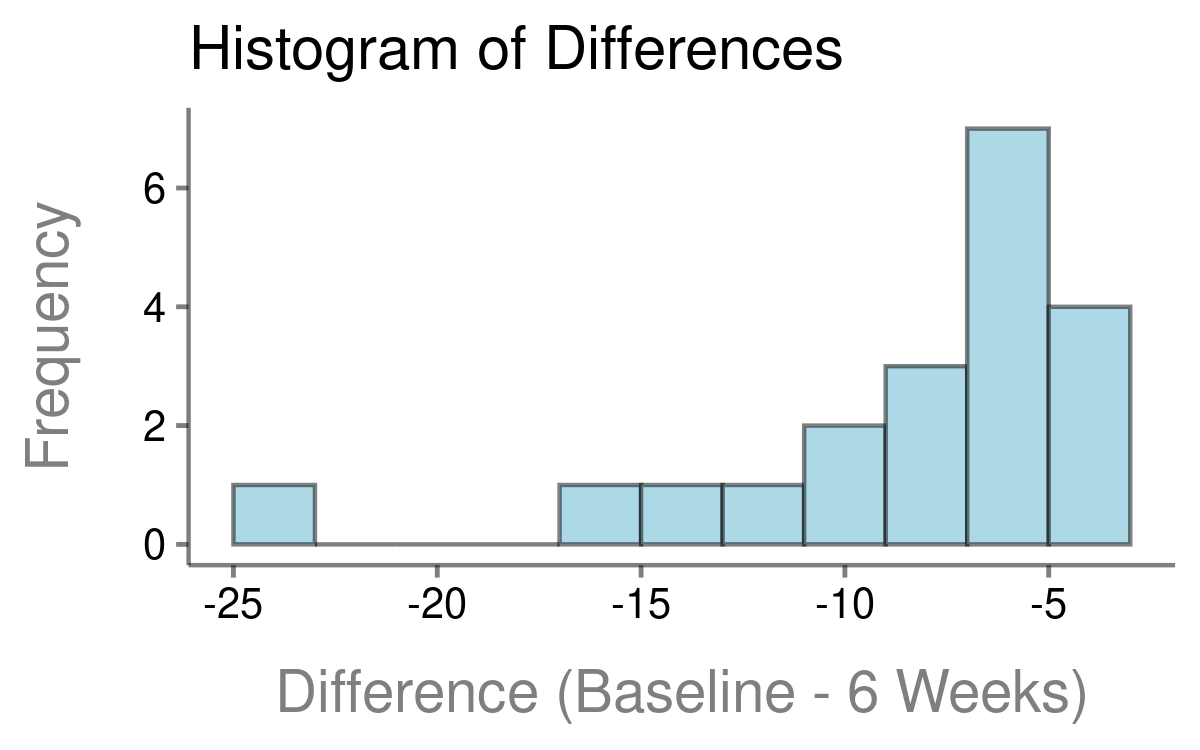
\includegraphics{DH302_Spring2025_Assignment02_files/figure-pdf/unnamed-chunk-19-1.png}

\begin{Shaded}
\begin{Highlighting}[]
\CommentTok{\# plotting qq plot}

\FunctionTok{qqnorm}\NormalTok{(data}\SpecialCharTok{$}\NormalTok{diff)}
\FunctionTok{qqline}\NormalTok{(data}\SpecialCharTok{$}\NormalTok{diff, }\AttributeTok{col =} \StringTok{"green"}\NormalTok{)}
\end{Highlighting}
\end{Shaded}

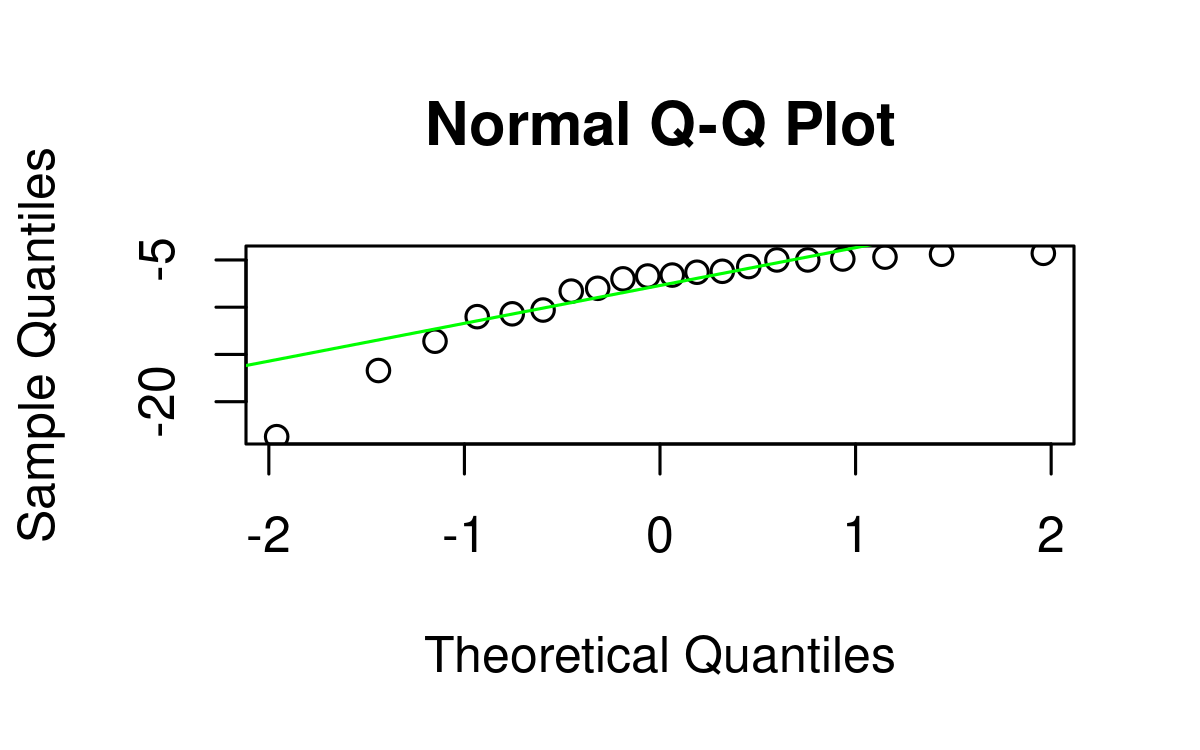
\includegraphics{DH302_Spring2025_Assignment02_files/figure-pdf/unnamed-chunk-20-1.png}

\paragraph{5d. Perform a test (using R) to test your hypothesis in a)
reporting p-value and the conclusion. {[}5
points{]}}\label{d.-perform-a-test-using-r-to-test-your-hypothesis-in-a-reporting-p-value-and-the-conclusion.-5-points}

\begin{Shaded}
\begin{Highlighting}[]
\CommentTok{\# CODE}

\NormalTok{test\_stat }\OtherTok{\textless{}{-}} \FunctionTok{t.test}\NormalTok{(data}\SpecialCharTok{$}\NormalTok{baseline, data}\SpecialCharTok{$}\NormalTok{measured\_6weekslater, }
                        \AttributeTok{paired =} \ConstantTok{TRUE}\NormalTok{, }\AttributeTok{alternative =} \StringTok{"greater"}\NormalTok{)}
\NormalTok{p\_value }\OtherTok{\textless{}{-}}\NormalTok{ test\_stat}\SpecialCharTok{$}\NormalTok{p.value}
\FunctionTok{print}\NormalTok{(p\_value)}
\end{Highlighting}
\end{Shaded}

\begin{verbatim}
[1] 0.9999999
\end{verbatim}

\textbf{p-value:} The p-value of the test is 0.9999999.

\textbf{Conclusion:} There is no evidence that grip strength decreased
after 6 weeks from breaking their wrists.

\paragraph{5e. Non parameteric test {[}5
points{]}}\label{e.-non-parameteric-test-5-points}

A class of tests we did not discuss in detail in class are
non-parameteric tests. We did discuss them in this
\href{https://docs.google.com/presentation/d/15kxh03hVBR1ybnuBBvbT5pfInju1IVkmVH1trWbKJn4/edit\#slide=id.g200cc23746fa5c2a_79}{slide}.
Using hints from the slide, perform a relevant non-parameteric test
(using R) for testing your hypothesis in a) and report the pvalue and
conclusion

\begin{Shaded}
\begin{Highlighting}[]
\CommentTok{\# YOUR RESPONSE HERE}
\NormalTok{test\_stat }\OtherTok{\textless{}{-}} \FunctionTok{wilcox.test}\NormalTok{(data}\SpecialCharTok{$}\NormalTok{baseline, data}\SpecialCharTok{$}\NormalTok{measured\_6weekslater, }
                                  \AttributeTok{paired =} \ConstantTok{TRUE}\NormalTok{, }\AttributeTok{alternative =} \StringTok{"greater"}\NormalTok{)}
\NormalTok{p\_value }\OtherTok{\textless{}{-}}\NormalTok{ test\_stat}\SpecialCharTok{$}\NormalTok{p.value}
\FunctionTok{print}\NormalTok{(p\_value)}
\end{Highlighting}
\end{Shaded}

\begin{verbatim}
[1] 1
\end{verbatim}

\textbf{Conclusion:} Since the data is paired and we are willing to
perform a non-parametric test, we did Wilcoxon signed rank test as shown
in the slides. The p-value is 1, this means that we have no evidence to
reject the null hypothesis.

\paragraph{5f. Transform the original variable by a log() transformation
and repeat your analysis in 5c and 5d {[}10
points{]}}\label{f.-transform-the-original-variable-by-a-log-transformation-and-repeat-your-analysis-in-5c-and-5d-10-points}

\begin{Shaded}
\begin{Highlighting}[]
\CommentTok{\# YOUR RESPONSE HERE}

\CommentTok{\# dataset has one entry as 0, i am makinng it 0.1, so as to compute log}
\NormalTok{data}\SpecialCharTok{$}\NormalTok{baseline[data}\SpecialCharTok{$}\NormalTok{baseline }\SpecialCharTok{==} \DecValTok{0}\NormalTok{] }\OtherTok{\textless{}{-}} \FloatTok{0.1}
\NormalTok{data}\SpecialCharTok{$}\NormalTok{measured\_6weekslater[data}\SpecialCharTok{$}\NormalTok{measured\_6weekslater }\SpecialCharTok{==} \DecValTok{0}\NormalTok{] }\OtherTok{\textless{}{-}} \FloatTok{0.1}

\NormalTok{data}\SpecialCharTok{$}\NormalTok{log\_baseline }\OtherTok{\textless{}{-}} \FunctionTok{log}\NormalTok{(data}\SpecialCharTok{$}\NormalTok{baseline)}
\NormalTok{data}\SpecialCharTok{$}\NormalTok{log\_measured\_6weekslater }\OtherTok{\textless{}{-}} \FunctionTok{log}\NormalTok{(data}\SpecialCharTok{$}\NormalTok{measured\_6weekslater)}
\NormalTok{data}\SpecialCharTok{$}\NormalTok{log\_difference }\OtherTok{\textless{}{-}}\NormalTok{ data}\SpecialCharTok{$}\NormalTok{log\_baseline }\SpecialCharTok{{-}}\NormalTok{ data}\SpecialCharTok{$}\NormalTok{log\_measured\_6weekslater}
\end{Highlighting}
\end{Shaded}

\begin{Shaded}
\begin{Highlighting}[]
\FunctionTok{ggplot}\NormalTok{(data, }\FunctionTok{aes}\NormalTok{(}\AttributeTok{x =}\NormalTok{ log\_difference)) }\SpecialCharTok{+}
  \FunctionTok{geom\_histogram}\NormalTok{(}\AttributeTok{binwidth =} \DecValTok{1}\NormalTok{, }\AttributeTok{fill =} \StringTok{"lightblue"}\NormalTok{, }
                 \AttributeTok{color =}\NormalTok{ scales}\SpecialCharTok{::}\FunctionTok{alpha}\NormalTok{(}\StringTok{"black"}\NormalTok{, }\FloatTok{0.5}\NormalTok{)) }\SpecialCharTok{+}
  \FunctionTok{ggtitle}\NormalTok{(}\StringTok{"Histogram of Differences"}\NormalTok{) }\SpecialCharTok{+}
  \FunctionTok{xlab}\NormalTok{(}\StringTok{"Difference (log(Baseline) {-} log(6 Weeks))"}\NormalTok{) }\SpecialCharTok{+}
  \FunctionTok{ylab}\NormalTok{(}\StringTok{"Frequency"}\NormalTok{) }\SpecialCharTok{+}
\NormalTok{  theme}
\end{Highlighting}
\end{Shaded}

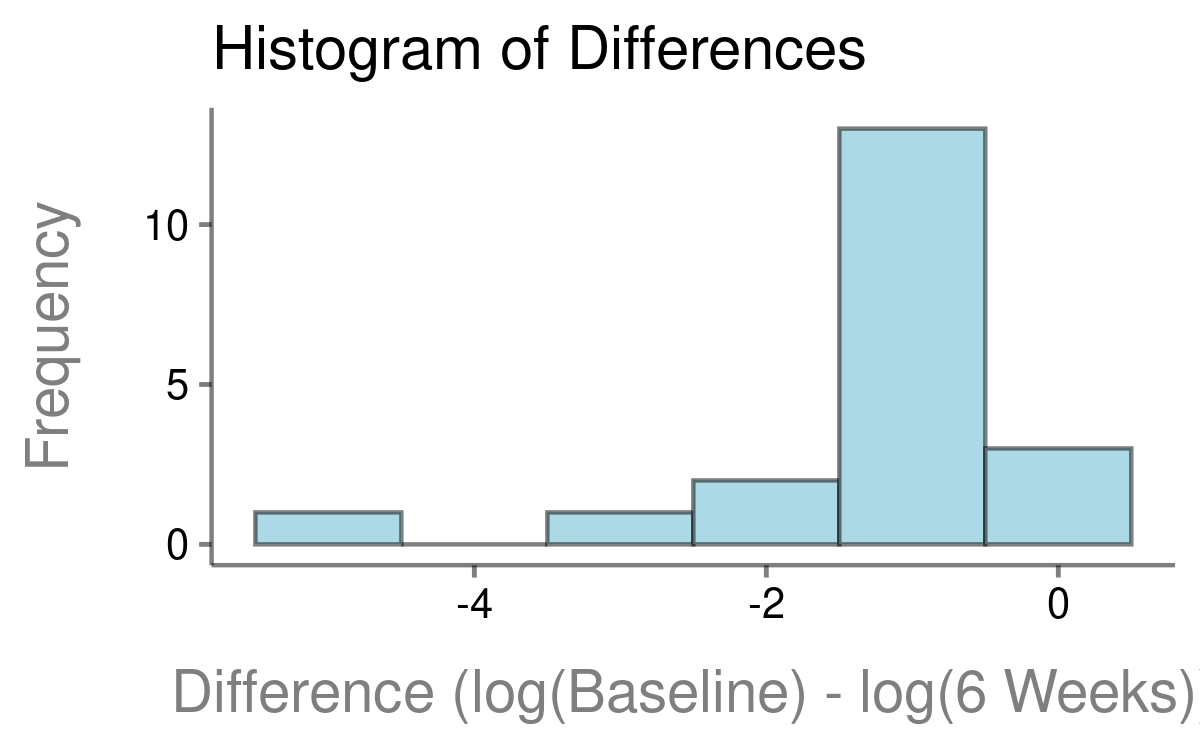
\includegraphics{DH302_Spring2025_Assignment02_files/figure-pdf/unnamed-chunk-24-1.png}

\begin{Shaded}
\begin{Highlighting}[]
\FunctionTok{qqnorm}\NormalTok{(data}\SpecialCharTok{$}\NormalTok{log\_difference)}
\FunctionTok{qqline}\NormalTok{(data}\SpecialCharTok{$}\NormalTok{log\_difference, }\AttributeTok{col =} \StringTok{"green"}\NormalTok{)}
\end{Highlighting}
\end{Shaded}

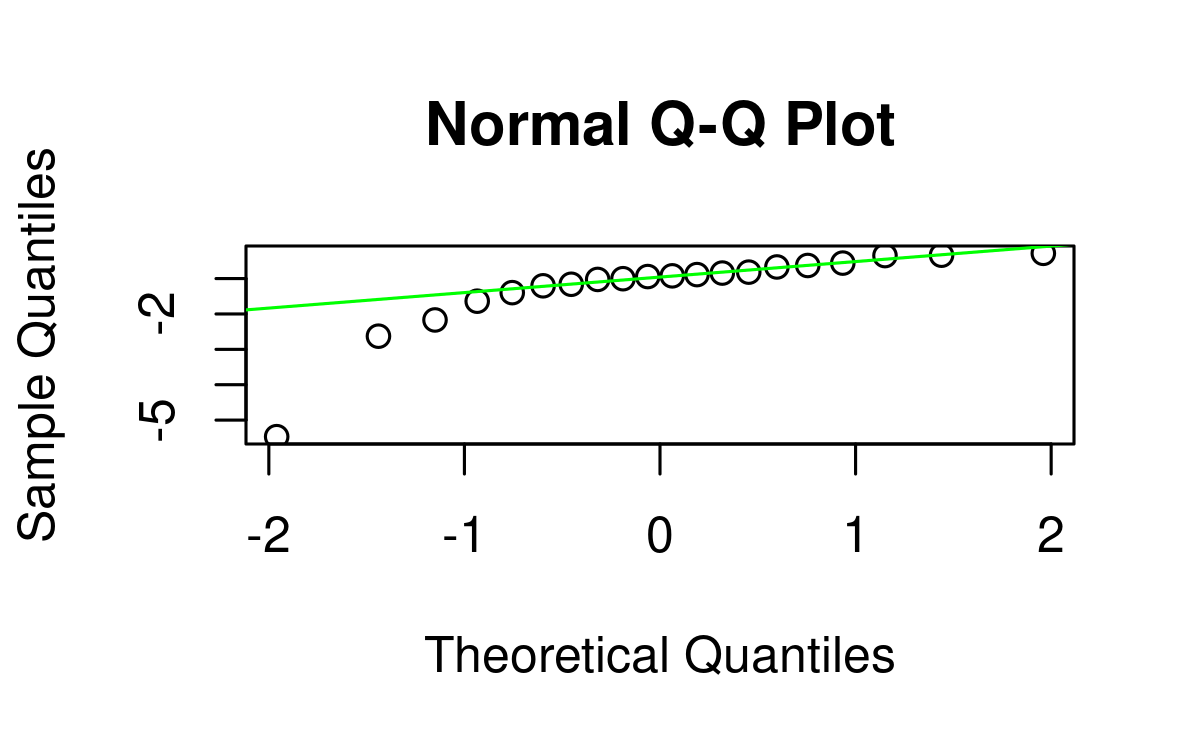
\includegraphics{DH302_Spring2025_Assignment02_files/figure-pdf/unnamed-chunk-25-1.png}

\begin{Shaded}
\begin{Highlighting}[]
\CommentTok{\# YOUR CODE HERE}
\NormalTok{test\_stat }\OtherTok{\textless{}{-}} \FunctionTok{t.test}\NormalTok{(data}\SpecialCharTok{$}\NormalTok{log\_baseline, data}\SpecialCharTok{$}\NormalTok{log\_measured\_6weekslater, }
                        \AttributeTok{paired =} \ConstantTok{TRUE}\NormalTok{, }\AttributeTok{alternative =} \StringTok{"greater"}\NormalTok{)}
\NormalTok{p\_value }\OtherTok{\textless{}{-}}\NormalTok{ test\_stat}\SpecialCharTok{$}\NormalTok{p.value}
\FunctionTok{print}\NormalTok{(p\_value)}
\end{Highlighting}
\end{Shaded}

\begin{verbatim}
[1] 0.9999426
\end{verbatim}

\textbf{p-value:} 0.9999426

\textbf{Conclusion:} We still don't have any evidence to reject the null
hypothesis.

Question: how does the result of your analysis compare with your
conclusion in d?

The p-value we got in (d) part is \textbf{greater} than what we got in
this part. From the qq plot we can see that the data this time is
\textbf{more normal}, and hence we can say that this normality made the
test more accurate, resulting in slight decrement in the p-value.

\section{Problem 06 {[}50 points{]}}\label{problem-06-50-points}

\textbf{PPT - Principal proteins test:} This is a data heavy question
and designed to give you another exposure to real world data which is
messy, hard to parse and often not so well documented. It is also to
tell you how a random (or not so random)
\href{https://x.com/sayajiraogaikwa/status/1887786728477573385}{twitter/X
thread} can be turned into an assignment problem - which is one of the
reasons the assignment was delayed (the other one being figuring out how
to combat ChatGPT usage for direct copy pasting answers (not code) ). It
is also to applaud the government of India for the wealth of data it
collects - you just need to find(parse) it.

The tsv
\href{https://drive.google.com/file/d/1e4eApFj1YbTgzPuIv9KK0TyJtKsG_5JO/view?usp=sharing}{here}
has the amino acid content of different food items. The data was
programmatically extracted from
\href{https://drive.google.com/file/d/1RqxhUezG2CXeufPvz59KY24B2VwKd7ED/view?usp=sharing}{this
PDF} and contains the amino acid profile of various food items - some
familar and some not so familiar ones. Very few people (in the world)
have taken a look at this data in the way you are going to.

Using dimensionality reduction techniques we studied in the
\href{https://saket-choudhary.me/DH302/syllabus.html}{class}, perform an
exploratory analysis and build a story around your plot. While the
question is broad, there are full points only for specific answers. The
questions are broad, but your responses should be specific.

\paragraph{\texorpdfstring{6a. \textbf{The plot}. Plot the output of PCA
to demonstrate what the lower dimensional representation of the data
looks like. {[}10
points{]}}{6a. The plot. Plot the output of PCA to demonstrate what the lower dimensional representation of the data looks like. {[}10 points{]}}}\label{a.-the-plot.-plot-the-output-of-pca-to-demonstrate-what-the-lower-dimensional-representation-of-the-data-looks-like.-10-points}

Remember the dataset is messy, if you want to do dimensionality
reduction, you want to only retain numeric columns. While the
\href{https://drive.google.com/file/d/1e4eApFj1YbTgzPuIv9KK0TyJtKsG_5JO/view?usp=sharing}{original
tsv} also has uncertainity, to make the task easier I have generated a
cleaned version of the tsv
\href{https://drive.google.com/file/d/1rKkfJO2unnTGvBRpKLPi-jnMnYEnKCCb/view?usp=sharing}{here}
removing the uncertainity values. There are 21 columns in total:

\begin{enumerate}
\def\labelenumi{\arabic{enumi}.}
\tightlist
\item
  \texttt{food\_code} = a short code for different food items,
\item
  \texttt{food\_name} = long description of the food
\item
  \texttt{number\_of\_regions} = Number of sampling regions (this can be
  IGNORED for this question)
\item
  18 columns corresponding to the 18 out of 20 amino acids with absolute
  quantities for each
\end{enumerate}

\begin{Shaded}
\begin{Highlighting}[]
\CommentTok{\# YOUR CODE GOES HERE}
\CommentTok{\# OUTPUT: A reduced dimensional representation of your data}
\CommentTok{\# You can choose to color your data points on a specific variable of choice}
\CommentTok{\# the variable can either exist in data or can be extracted(appended) by}
\CommentTok{\# processing the data frame}
\NormalTok{df }\OtherTok{\textless{}{-}} \FunctionTok{read\_tsv}\NormalTok{(}\StringTok{"./Table8\_amino\_acid\_profile\_no\_uncertainity.tsv"}\NormalTok{)}
\end{Highlighting}
\end{Shaded}

\begin{verbatim}
Rows: 612 Columns: 39
-- Column specification --------------------------------------------------------
Delimiter: "\t"
chr  (2): food_code, food_name
dbl (37): number_of_regions, Alanine, Arginine, Aspartic Acid, Glutamic Acid...

i Use `spec()` to retrieve the full column specification for this data.
i Specify the column types or set `show_col_types = FALSE` to quiet this message.
\end{verbatim}

\begin{Shaded}
\begin{Highlighting}[]
\NormalTok{df }\OtherTok{\textless{}{-}}\NormalTok{ df }\SpecialCharTok{\%\textgreater{}\%}
  \FunctionTok{drop\_na}\NormalTok{() }\SpecialCharTok{\%\textgreater{}\%}
  \FunctionTok{unique}\NormalTok{() }\SpecialCharTok{\%\textgreater{}\%}
  \FunctionTok{as.data.frame}\NormalTok{()}
\end{Highlighting}
\end{Shaded}

\begin{Shaded}
\begin{Highlighting}[]
\CommentTok{\# we will reduce the dimension of data from 18 to 2, trying to keep variance}
\CommentTok{\# (information retention) as high as possible using PCA}
\FunctionTok{library}\NormalTok{(tidyverse)}
\FunctionTok{library}\NormalTok{(ggplot2)}
\FunctionTok{library}\NormalTok{(FactoMineR)}
\FunctionTok{library}\NormalTok{(factoextra)}
\end{Highlighting}
\end{Shaded}

\begin{verbatim}
Welcome! Want to learn more? See two factoextra-related books at https://goo.gl/ve3WBa
\end{verbatim}

\begin{Shaded}
\begin{Highlighting}[]
\NormalTok{df\_numeric }\OtherTok{\textless{}{-}}\NormalTok{ df[, }\DecValTok{4}\SpecialCharTok{:}\DecValTok{21}\NormalTok{] }
\NormalTok{df}\SpecialCharTok{$}\NormalTok{food\_category }\OtherTok{\textless{}{-}} \FunctionTok{substr}\NormalTok{(df}\SpecialCharTok{$}\NormalTok{food\_code, }\DecValTok{1}\NormalTok{, }\DecValTok{1}\NormalTok{)}
\NormalTok{pca\_result }\OtherTok{\textless{}{-}} \FunctionTok{PCA}\NormalTok{(df\_numeric, }\AttributeTok{scale.unit =} \ConstantTok{TRUE}\NormalTok{, }\AttributeTok{graph =} \ConstantTok{FALSE}\NormalTok{)}

\FunctionTok{fviz\_pca\_ind}\NormalTok{(pca\_result,}
             \AttributeTok{geom =} \StringTok{"point"}\NormalTok{,}
             \AttributeTok{addEllipses =} \ConstantTok{TRUE}\NormalTok{,}
             \AttributeTok{label =} \StringTok{"none"}\NormalTok{,}
             \AttributeTok{title =} \StringTok{"PCA of Amino Acid Profile of Foods"}\NormalTok{,}
             \AttributeTok{pointsize =} \DecValTok{3}\NormalTok{,}
             \AttributeTok{alpha.ind =} \FloatTok{0.5}\NormalTok{,}
             \AttributeTok{col.ind =} \StringTok{"steelblue"}\NormalTok{,}
             \AttributeTok{repel =} \ConstantTok{TRUE}\NormalTok{,}
\NormalTok{  ) }\SpecialCharTok{+}
  \FunctionTok{theme\_minimal}\NormalTok{() }\SpecialCharTok{+}
  \FunctionTok{theme}\NormalTok{(}\AttributeTok{plot.title =} \FunctionTok{element\_text}\NormalTok{(}\AttributeTok{size =} \DecValTok{14}\NormalTok{, }\AttributeTok{face =} \StringTok{"bold"}\NormalTok{)) }\SpecialCharTok{+}
  \FunctionTok{coord\_cartesian}\NormalTok{(}\AttributeTok{ylim =} \FunctionTok{c}\NormalTok{(}\SpecialCharTok{{-}}\DecValTok{8}\NormalTok{, }\DecValTok{5}\NormalTok{))}
\end{Highlighting}
\end{Shaded}

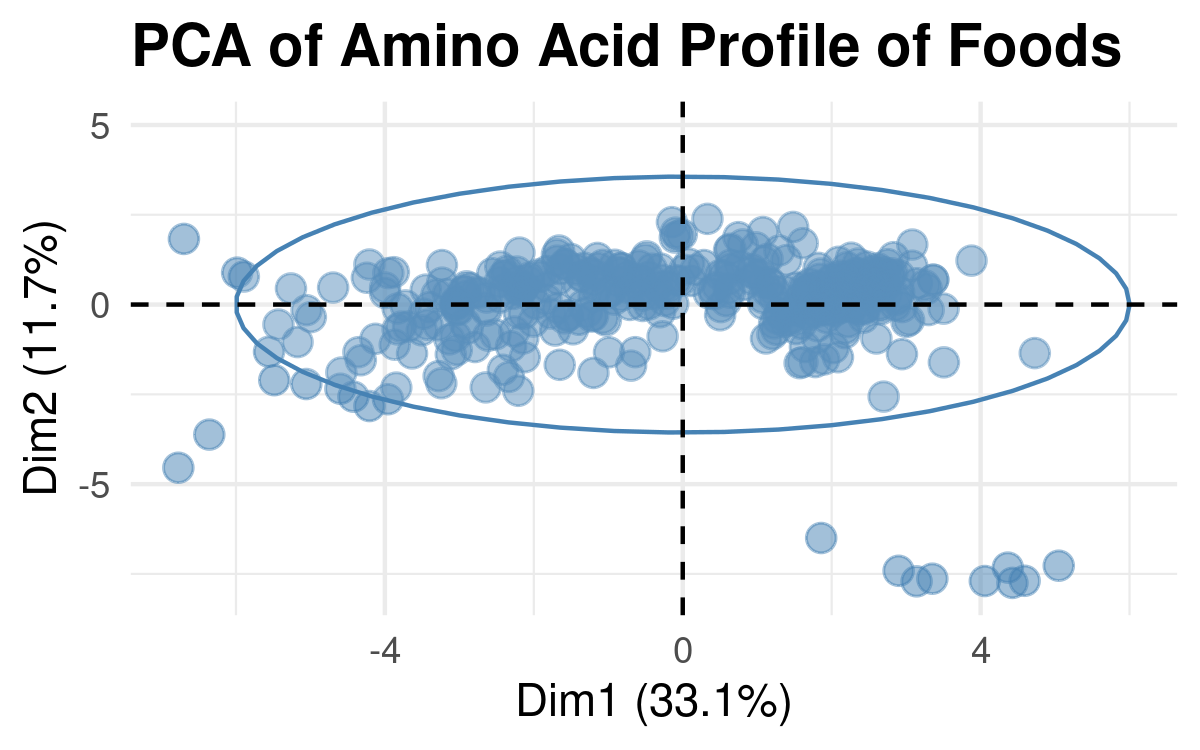
\includegraphics{DH302_Spring2025_Assignment02_files/figure-pdf/unnamed-chunk-28-1.png}

\paragraph{\texorpdfstring{6b. \textbf{The story} Do you notice any
discernible pattern in your data? What are some factor(s) that explain
your PC1 and PC2? {[}10
points{]}}{6b. The story Do you notice any discernible pattern in your data? What are some factor(s) that explain your PC1 and PC2? {[}10 points{]}}}\label{b.-the-story-do-you-notice-any-discernible-pattern-in-your-data-what-are-some-factors-that-explain-your-pc1-and-pc2-10-points}

\begin{Shaded}
\begin{Highlighting}[]
\CommentTok{\# WRITE ADDITIONAL CODE TO EXPLAIN YOUR STORY}
\CommentTok{\#}

\NormalTok{var\_contrib }\OtherTok{\textless{}{-}} \FunctionTok{get\_pca\_var}\NormalTok{(pca\_result)}
\FunctionTok{fviz\_pca\_var}\NormalTok{(pca\_result, }\AttributeTok{col.var =} \StringTok{"contrib"}\NormalTok{, }\AttributeTok{repel =} \ConstantTok{TRUE}\NormalTok{) }\SpecialCharTok{+}
\FunctionTok{scale\_color\_gradient2}\NormalTok{(}\AttributeTok{low =} \StringTok{"pink"}\NormalTok{, }\AttributeTok{mid =} \StringTok{"violet"}\NormalTok{, }\AttributeTok{high =} \StringTok{"blue"}\NormalTok{, }\AttributeTok{midpoint =} \FunctionTok{mean}\NormalTok{(var\_contrib}\SpecialCharTok{$}\NormalTok{contrib)) }\SpecialCharTok{+}
\NormalTok{  theme}
\end{Highlighting}
\end{Shaded}

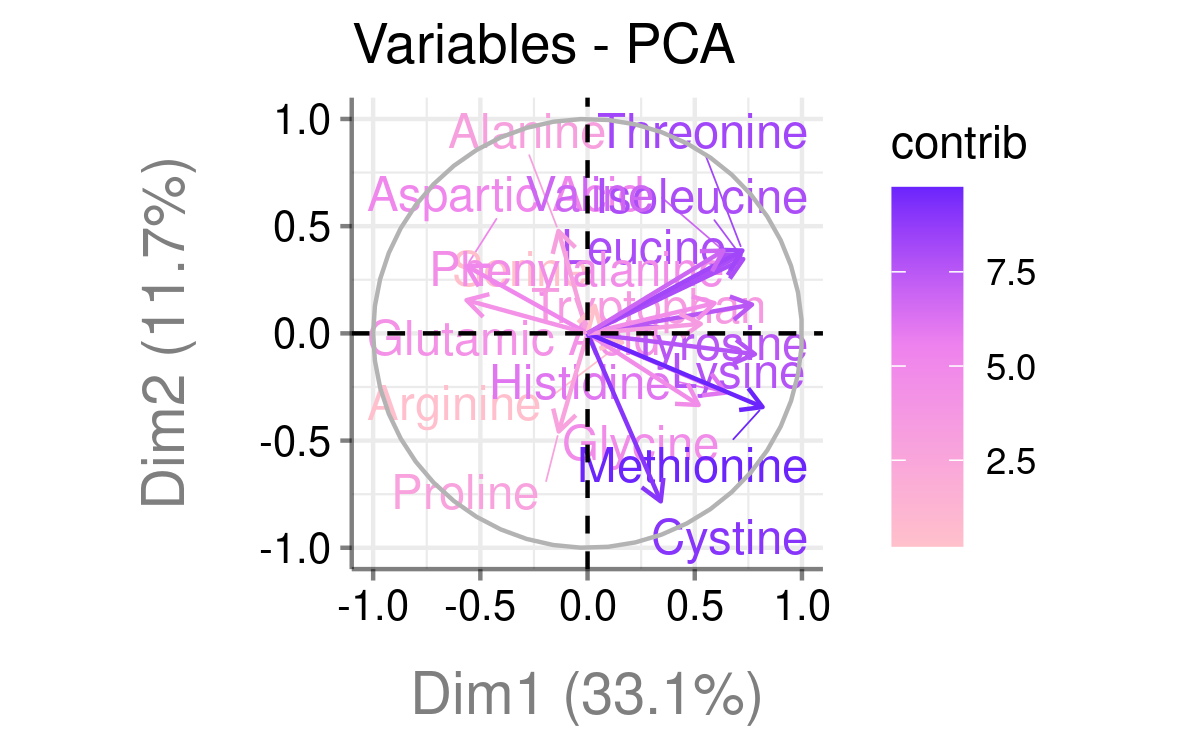
\includegraphics[width=0.9\textwidth]{DH302_Spring2025_Assignment02_files/figure-pdf/unnamed-chunk-29-1.png}

\begin{itemize}
\item
  PC1 might be differentiating the food on the basis of their pH levels,
  since acidic amino acids are at one side of the axis and non-acidic
  are at the other side. Or the PC1 may be classifying the food basis of
  the total protein content. Low protein food is on the left side of the
  axis, while high protein food on the right side.
\item
  PC2 may capture differences related to polarity and specific side
  chain properties. Hydrophobic amino acids are at the top, while more
  polar or structurally unique amino acids are at the bottom. PC2 may
  also be capturing differences in structural flexibility, highly
  flexible amino acids like glycine are at the lower side, while rigid
  amino acids like valine and leucine are at the upper side.
\end{itemize}

\subsubsection{\texorpdfstring{6c. \textbf{The factors} Identify the top
2 factors (features) that are associated with your PC1 and that with
PC2. {[}15
points{]}}{6c. The factors Identify the top 2 factors (features) that are associated with your PC1 and that with PC2. {[}15 points{]}}}\label{c.-the-factors-identify-the-top-2-factors-features-that-are-associated-with-your-pc1-and-that-with-pc2.-15-points}

\begin{Shaded}
\begin{Highlighting}[]
\CommentTok{\# WRITE ADDITIONAL CODE TO SHOW FACTORS ASSOCIATED WITH PC1 and PC2}
\CommentTok{\#}

\NormalTok{var\_contrib }\OtherTok{\textless{}{-}} \FunctionTok{get\_pca\_var}\NormalTok{(pca\_result)}\SpecialCharTok{$}\NormalTok{contrib}

\NormalTok{topPC1 }\OtherTok{\textless{}{-}}\NormalTok{ var\_contrib[}\FunctionTok{order}\NormalTok{(}\SpecialCharTok{{-}}\NormalTok{var\_contrib[,}\DecValTok{1}\NormalTok{]), ][}\DecValTok{1}\SpecialCharTok{:}\DecValTok{2}\NormalTok{, ]}
\NormalTok{topPC2 }\OtherTok{\textless{}{-}}\NormalTok{ var\_contrib[}\FunctionTok{order}\NormalTok{(}\SpecialCharTok{{-}}\NormalTok{var\_contrib[,}\DecValTok{2}\NormalTok{]), ][}\DecValTok{1}\SpecialCharTok{:}\DecValTok{2}\NormalTok{, ]}

\FunctionTok{print}\NormalTok{(}\StringTok{"Top 2 features for PC1:"}\NormalTok{)}
\end{Highlighting}
\end{Shaded}

\begin{verbatim}
[1] "Top 2 features for PC1:"
\end{verbatim}

\begin{Shaded}
\begin{Highlighting}[]
\FunctionTok{print}\NormalTok{(topPC1)}
\end{Highlighting}
\end{Shaded}

\begin{verbatim}
              Dim.1     Dim.2     Dim.3     Dim.4     Dim.5
Methionine 11.19196 5.6246906 0.2070543 0.4254628 0.1554596
Lysine     10.23655 0.4471709 3.1782960 0.1114583 0.1380230
\end{verbatim}

\begin{Shaded}
\begin{Highlighting}[]
\FunctionTok{cat}\NormalTok{(}\StringTok{"}\SpecialCharTok{\textbackslash{}n\textbackslash{}n}\StringTok{"}\NormalTok{)}
\end{Highlighting}
\end{Shaded}

\begin{Shaded}
\begin{Highlighting}[]
\FunctionTok{print}\NormalTok{(}\StringTok{"Top 2 features for PC2:"}\NormalTok{)}
\end{Highlighting}
\end{Shaded}

\begin{verbatim}
[1] "Top 2 features for PC2:"
\end{verbatim}

\begin{Shaded}
\begin{Highlighting}[]
\FunctionTok{print}\NormalTok{(topPC2)}
\end{Highlighting}
\end{Shaded}

\begin{verbatim}
            Dim.1    Dim.2      Dim.3       Dim.4      Dim.5
Cystine 1.9588305 29.24931  0.1978986  0.07728457 0.03527014
Alanine 0.3094629 10.87089 11.1356048 14.02252684 2.36862851
\end{verbatim}

\begin{itemize}
\item
  The amino acids contributing maximum towards PC1 are:
  \textbf{Methionine} and \textbf{Lysine}.
\item
  The amino acids contributing maximum towards PC2 are: \textbf{Cystine}
  and \textbf{Alanine}.
\end{itemize}

\subsubsection{\texorpdfstring{6d. \textbf{Is it statistically
significant?} Based on the topmost factor that you identified in 6c for
PC1, perform a statistical test to test if this factor is statistically
different between the two groups you identified in c.~To define the two
groups you can make use of the \texttt{code\_desc} column (HINT:
Individual food codes are not so useful but categories probably are)
{[}15
points{]}}{6d. Is it statistically significant? Based on the topmost factor that you identified in 6c for PC1, perform a statistical test to test if this factor is statistically different between the two groups you identified in c.~To define the two groups you can make use of the code\_desc column (HINT: Individual food codes are not so useful but categories probably are) {[}15 points{]}}}\label{d.-is-it-statistically-significant-based-on-the-topmost-factor-that-you-identified-in-6c-for-pc1-perform-a-statistical-test-to-test-if-this-factor-is-statistically-different-between-the-two-groups-you-identified-in-c.-to-define-the-two-groups-you-can-make-use-of-the-code_desc-column-hint-individual-food-codes-are-not-so-useful-but-categories-probably-are-15-points}

\begin{Shaded}
\begin{Highlighting}[]
\CommentTok{\# YOUR CODE HERE}
\end{Highlighting}
\end{Shaded}





\end{document}
